\documentclass[11pt,a4paper]{article}
\usepackage[latin1]{inputenc}
\usepackage{amsmath}
\usepackage{pdflscape}
\usepackage{rotating}
\usepackage{amsfonts}
\usepackage{tabu}
\usepackage{cite}

\numberwithin{equation}{subsection}
\usepackage[titletoc]{appendix}
\usepackage{amssymb}
\usepackage{graphicx}
\usepackage{tabularx}
\usepackage{caption}
\usepackage{multirow}
\usepackage{setspace}
\usepackage{fancyhdr}
\usepackage[export]{adjustbox}
%\usepackage{floatrow}
%\usepackage[singlelinecheck=off]{caption}
\DeclareRobustCommand\nocite[1]{%
	{\def\cite##1{\ignorespaces}#1}}
\newcommand\nocitecaption[1]{\caption[\nocite{#1}]{#1}}

% Set folder for images
\graphicspath{ {Figures_and_Images/} }

% Set Margins
\usepackage{geometry}
\geometry{, total={145mm,247mm}, left = 40mm, top = 25mm}

% Set Font
\usepackage{pslatex} %Times font

% Set up Left Align Table Caption
 \captionsetup[table]{
 	labelsep = newline, 
 	name = Table, 
 	justification=justified,
 	singlelinecheck=false,%%%%%%% a single line is centered by default
 	labelsep=colon,%%%%%%
 	skip = \bigskipamount}
 
  \captionsetup[figure]{
  	labelsep = newline, 
  	name = Figure, 
  	justification=justified,
  	singlelinecheck=true,%%%%%%% a single line is centered by default
  	labelsep=colon,%%%%%%
  	skip = \bigskipamount}


%--------------------------------------------------------------
%	TITLE PAGE
%--------------------------------------------------------------
\thispagestyle{empty}

\newcommand*{\titleGP}{\begingroup % Create the command for including the title page in the document
	\centering % Center all text
	\vspace*{\baselineskip} % White space at the top of the page
	
	
	{\Large JAMES COOK UNIVERSITY\\ [0.3\baselineskip] } % Title
	
	{\Huge COLLEGE OF SCIENCE \&{} ENGINEERING\\ [0.3\baselineskip] } % Title
	
	\vspace*{7\baselineskip} % Whitespace between location/year and editors
	
	{\Huge EG4011\\ Civil Engineering\\ [0.3\baselineskip] } % Title
	
	\vspace*{6\baselineskip} % Whitespace between location/year and editors
	
	{\Huge \bf{STRENGTHENING OF NOTCHED CIRCULAR TIMBER GIRDERS USING FIBRE REINFORCED POLYMERS}\\ [0.3\baselineskip] } % Title
	
	\vspace*{2\baselineskip} % Whitespace between location/year and editors
	
	{\LARGE LARA MULLAMPHY\par} % Editor list

	
	\vfill % Whitespace between editor names and publisher logo
	
	
		\scshape % Small caps
		Proposal submitted to the School of Engineering and Physical Sciences in partial fulfilment of the requirements for the degree of \\
		{\Large Bachelor of Engineering\\ (Civil Engineering)} % Tagline(s) or further description
		\\[\baselineskip] % Tagline(s) or further description
		29 April 2016\par % Location and year
	
	\endgroup}

%--------------------------------------------------------------

\begin{document}

%------------------------- Title Page -------------------------
	\titleGP % This command includes the title page

	% Set Line Spacing to 1.5
	\setstretch{1.5}
	
	\pagestyle{fancy}
%	\thispagestyle{empty}
	\fancyhead{}
	\fancyfoot{}
	\renewcommand{\headrulewidth}{0pt}
	\fancyfoot[R]{\thepage}
	\pagenumbering{roman}
	\pagebreak
%-------------------- Statement of Access -----------------------
% See Thesis manual

%-------------------- Declaration of Sources -------------------

% See Thesis manual

%-------------------- Table of Contents -------------------	 
	\tableofcontents
	\vspace*{\baselineskip}
	\vspace*{\baselineskip}
	
	\pagebreak

	\nocite\listoffigures 
	\addcontentsline{toc}{section}{List of Figures}
	\listoftables
	\addcontentsline{toc}{section}{List of Tables}
	\pagebreak
	
%---------------------- Introduction --------------------------
	\section{Introduction}
	
	\pagenumbering{arabic}
	\setcounter{page}{1}
	% State the general topic

	
	\noindent
	Timber has been a dominant material in engineering and construction for centuries and continues to be a major material used in housing, floors and furniture. Timber was also the first material used to construct bridges and, although it is slowly being replaced by alternative building materials, there are currently around 20,000 timber road bridges still currently in use within Australia. Many of the bridges still in use are utilised by rail \cite{wilkinson_capacity_2008} which is subject to significant load and hence the maintenance and strengthening of these bridges is of major importance. 
    
    \vspace*{\baselineskip}
    
    \noindent
    Over the past few decades there has been a major decrease in the use of timber for the construction of bridges. This is predominately due to the inherent properties of timber which expose it to environmental problems such as weathering, rotting and insect infestation. These conditions make the bridge expensive to maintain and significantly limits the lifespan of the structure.  Hence the majority of bridges now being constructed in Queensland utilise steel and concrete to minimize the impact of any environmental damage. However, many timber bridges throughout Queensland still remain in use and hence require regular maintenance and strengthening to withstand growing load demands and remain stable until they are eventually replaced. As the complete replacement of bridges is expensive, the alternative of strengthening the structure appears to be the more feasible option. One of the primary sections of timber bridges which require strengthening are the notches in the timber beams. These sections are particularly prone to cracking and need to be studied in order to find a suitable method for strengthening these regions.
	
	\vspace*{\baselineskip}
	
	\noindent
     Notching is when a section from a member is cut out to ease insertion and act as seating for timber girders over piers or abutments. This is common practice in the construction of timber bridges and places increased risk of failure to the structure at the position of the notches.This increased risk occurs due the section loss from notching exposing the timber to the risk of cracking and potential failure. As notches reduce beam capacities, the need to strengthen this area is of high importance. Currently there is little information on notching design surrounding circular members or evaluating capacities of a notched round member. This is of significant importance in the construction of timber bridges as most members currently used in bridges are round. A study of the literature has revealed that there have been very few studies carried out on the strengthening of these notches in circular section beams. Hence there remains a strong need for further investigation, with a particular emphasis for the strengthening of notches in circular members used in the construction of timber bridges. 
	
	\vspace*{\baselineskip}
	
	\noindent
    The proposed research will provide further understanding into the effects of notches and notch angles on round timber members. Current notch design methods will be investigated and compared to determine which method obtains the most accurate results. As many bridges are currently suffering issues caused by notching, the ability to understand the effects of notching will assist in a further understanding of how to design and possibly strengthen them. By establishing an effective method of notch design, 
    %increase their lifespan and delay the need for total replacement will be of significant importance to reducing the overall costs associated with timber bridges.  
	
	
	\subsection{Objectives}
	The aim of this research is to determine the structural behaviour of circular section timber girders with different notched angles. Using these results, methods of strengthening the notched girders using FRP can be tested. The main objectives of this research are to:\par 
	
	\begin{enumerate}
		\item Determine the effects of different notch types on the flexural and shear capacity of rectangular and circular timber beams
		\item Validate existing design equations for notched timber girders
		\item Develop a finite element analysis model to simulate the behaviour of both strengthened and un-strengthened notched timber girders.
	\end{enumerate}
	
	\subsection{Scope}
	\noindent
	The overall scope of this research is to determine the effects of notching on rectangular and circular section members. This will be achieved through small-scale experiments where notch angles will be altered on both section types.
	
	\pagebreak
	
	\section{Literature Review}
	
	\subsection{Timber Bridges}
	Timber has been used in the construction of bridges for thousands of years \cite{ritter_timber_1990} and remained the preferred construction material until the middle of the 20th century when it was eventually replaced by the introduction of steel and concrete \cite{ritter_timber_1990,_timber_2005} . Timber had remained the dominant building material because of its strength and light weight. Timber also has energy- absorbing properties, making it capable of handling short term overloads without harmful effects, making it an excellent material for bridge construction. Large timber members also have good fire resistance qualities, are relatively durable and have the ability to withstand de-icing effects. Overall the construction of timber bridges is very cost effective as timber is a relatively cheap and renewable resource and installation can usually be carried out without the need of heavy machinery, significantly reducing the labour required \cite{ritter_timber_1990}. Although timber bridges are relatively cost effective to build, susceptibility to weather and insects make them expensive to maintain.
	
	\vspace*{\baselineskip}
	
	\noindent
	Ongoing repairs for the timber structure can be labour intensive and expensive, hence preventative maintenance is important in cutting costs and prolonging the life of the bridge. To prevent deterioration, the timber can be chemically treated against damage to weathering from sunlight exposure and moisture. This is a major benefit as there is little to no maintenance or painting required for wood treated with preservatives \cite{ritter_timber_1990}. Furthermore, the wood can be treated to prevent pest infestation \cite{_timber_2005,ritter_timber_1990} which can cause major damage to any timber structure. The commonplace use of chemical treatment to preserve timber bridges has almost certainly added decades to the life of the bridge. However, when significant damage has already occurred, strengthening may be the only feasible option to prevent further damage and eventual failure of the bridge.
	
	\vspace*{\baselineskip}
	
	\noindent
	The availability of suitable timber is now a major concern for existing timber bridges which require substantial maintenance throughout their structural life \cite{_timber_2005}. The ability to source large sections of wood and sawn timber is becoming increasingly more difficult as the amount of timber suitable for harvesting decreases over time. The drive for forest preservation has also increased, heavily reducing the amount of suitable timber needed for bridge construction and maintenance \cite{_timber_2005,ritter_timber_1990}. This is another strong reason for strengthening current structures as the raw materials required for repair or replacement of timber bridges are costly and difficult to source.
	
	\subsubsection{Wood Types}
	There are two classes of timber; hardwood and softwood. The two types of wood can initially be distinguished by their leaves as hardwood trees have broad leaves and softwood trees have sharp needle like foliage \cite{dunningham_review_2015}. 
	
	\vspace*{\baselineskip}
	
	\noindent
	The major difference between hardwood and softwood is their cell structures \cite{stalnaker_structural_2013}. Hardwood contains mainly fibres, vessels/pores and parenchymas whereas softwoods contain tracheids (early- and latewood), resin canals and parenchymas \cite{cresswell_product_2004}.
	
	\vspace*{\baselineskip}
	
	\noindent
	It can be seen in Figure \ref{fig:Wood} that the cell structure of hardwood is substantially more complex than softwood \cite{mohanty_natural_2005}. The cell structure of softwood has a organised arrangement, whereas the cell arrangement of hard wood appears more random. A common misconception is that hardwood is hard in comparison to softwood, however this is not necessarily the case \cite{pipinato_innovative_2015,marshall_black_2005}. To determine whether to use softwood or hardwood, the major deciding factor is based on the intended purpose of the wood (i.e. whether it is to be in tension or compression).
	
		\begin{figure}[h]
			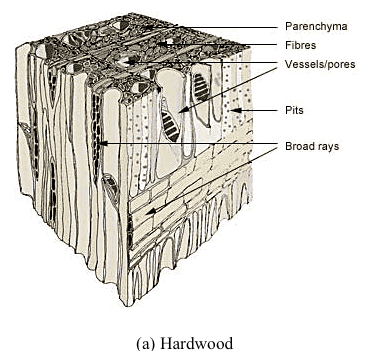
\includegraphics[scale=0.6]{Hardwoods}
			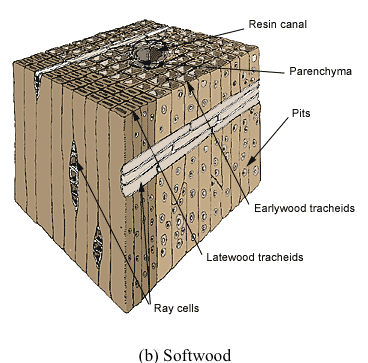
\includegraphics[scale=0.6]{Softwoods}	
			\caption{Wood Cell Structures \cite{_softwood_2016}}
			\label{fig:Wood}
		\end{figure}
	
	
	\noindent
	Table \ref{tab:Aspect} compares the aspect ratio of hardwood and softwood; these differ depending on the exact wood used and their particle/fibre size. From this it can be seen that generally hardwoods have a higher aspect ratio which implies they have better bending abilities, and thus are superior in sustaining tensile loads \cite{klyosov_wood-plastic_2007}. 
	
	\pagebreak
	\begin{center}
		\captionof{table}{Wood Cell Structures \cite{_softwood_2016}}
		\label{tab:Aspect}
		\begin{tabular}{c c c} 
			\hline
			\multirow{2}{*}{Particle size Range} & \multicolumn{2}{c}{Aspect Ratio} \\
			\cline{2-3}
			
			& Hardwoods & Softwoods \\ [0.5ex] 
			\hline
			20 mesh $(850\mu m - 0.85mm)$ & 4.6 & 3.5 \\ [0.5ex]
			
			40 mesh $(425\mu m - 0.425mm)$ & 4.4 & 3.4 \\ [0.5ex]
			
			60 mesh $(250\mu m - 0.25mm)$ & 4.4 & 4.2 \\ [0.5ex]
			
			800 mesh $(180\mu m - 0.18mm)$ & 4.2 & 4.5 \\ [0.5ex]
			
			\hline
			
		\end{tabular}
	\end{center}
	
	\vspace*{\baselineskip}
	
	\noindent
	More commonly used in timber bridge structures in Australia is hardwood due to its abundance at the time of construction\cite{rta_timber_2000}, as well its combination of high strength, durability, light-weight and most importantly flexural properties \cite{klyosov_wood-plastic_2007}. Commonly used woods in Queensland bridges are spotted gum, tally-wood and swamp mahogany. Spotted gum is strong, light-weight, tough, elastic and durable, and is particularly well-performing when in tension. Tally-wood is strong, durable and very tough; it withstands underground and aqueous conditions and is used mainly in decking and posts. Swamp mahogany is elastic, strong, tough and durable, which also sustains well in underground and aqueous conditions; it is predominately used in piles \cite{_queensland_1899}.
	
	\subsubsection{Common Defects and Failures}
    There are four major defects that are commonly occurring in timber bridges; weathering, rot- ting, cracking and termite infestation. These defects severely reduce the lifespan of a timber bridge and will all eventually lead to member failure.

    \vspace*{\baselineskip}
    
    \noindent
    \textbf{Weathering and Rotting}

	\noindent
	Weathering and rotting occur in timber members due to exposure to a combination of wind, wetting, drying and UV radiation \cite{_timber_2005,_section_2008}. The appearance of the weathering damage depends on the elements the timber is exposed to. Exposure to high wind speeds can cause dints/abrasions from small pebbles or embedded sand particles \cite{harrowfield_analysis_2006}, whereas exposure to a combination of running water and sun light can cause a ripple effect, as shown on a rail bridge longitudinal girder in the Figure \ref{fig:Weather}.
	
\begin{figure}[h]
	\begin{center}
		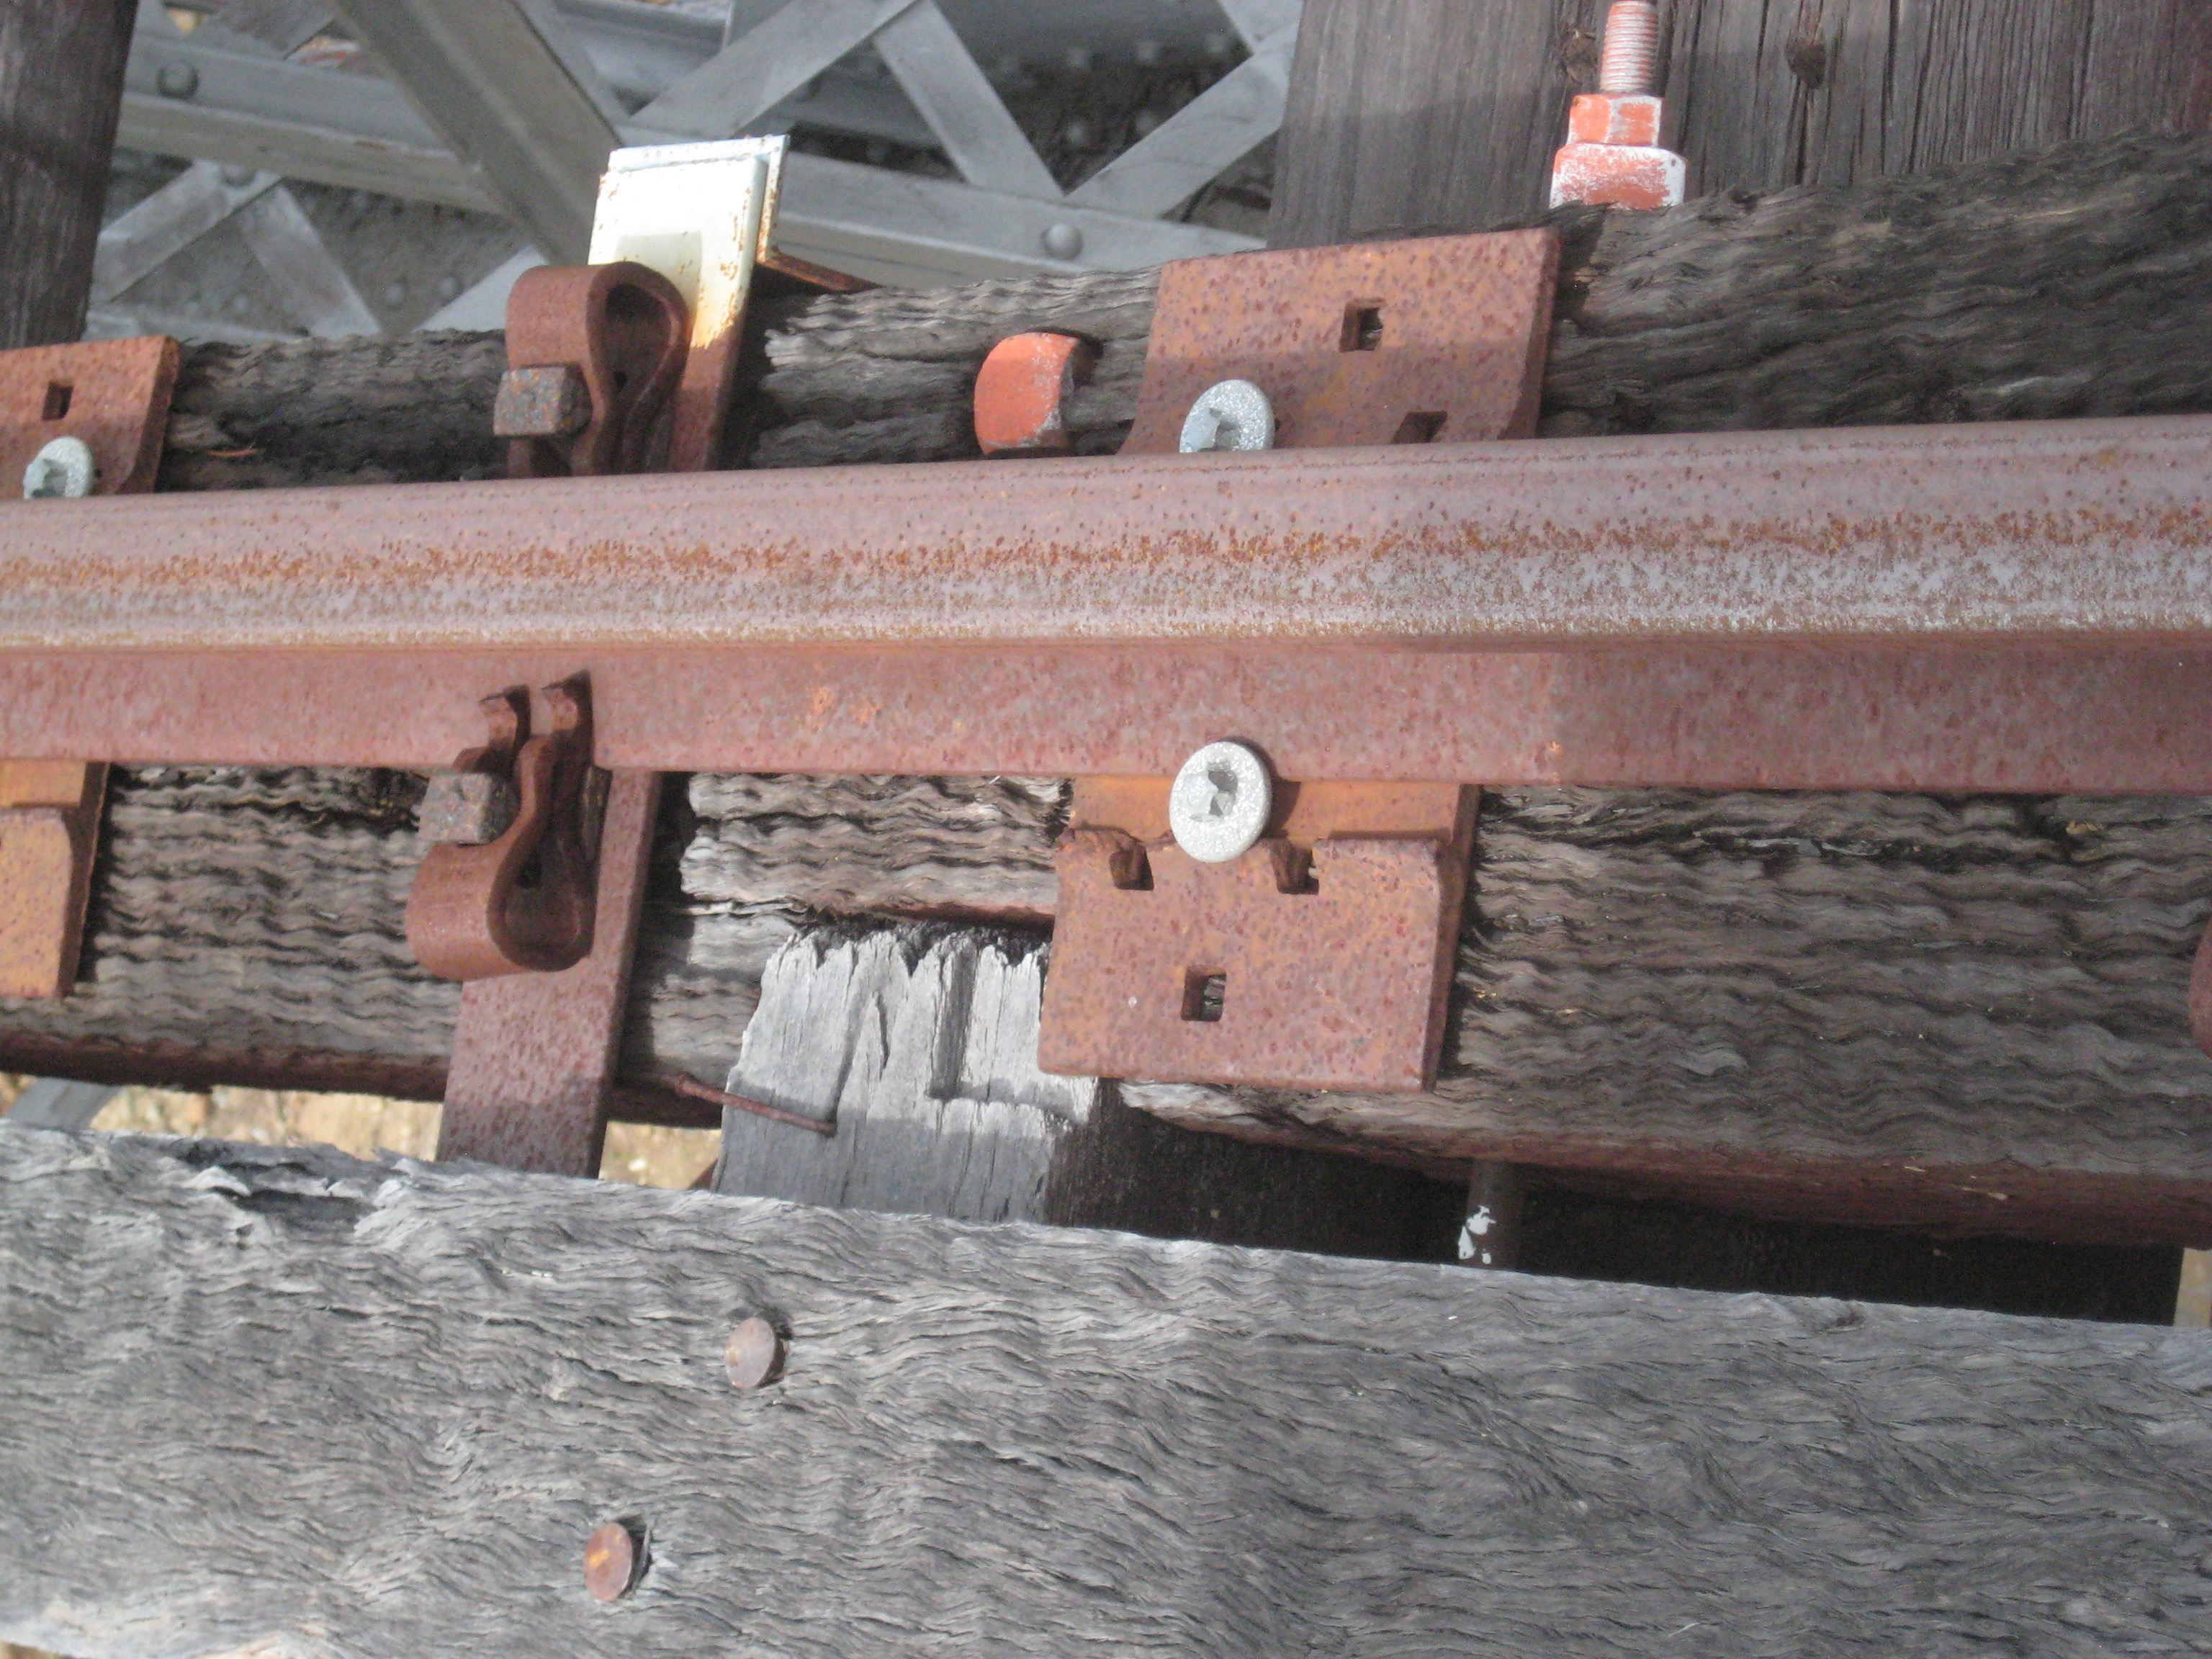
\includegraphics[scale=0.07]{Weathering}
	\end{center}
	\caption{Weathering}
	\label{fig:Weather}
\end{figure}
	\pagebreak
	
	 \noindent
	 Rotting occurs in areas where moisture is allowed to penetrate the wood and can lead to core rotting as shown in Figure \ref{fig:Rot} which severely reduces the strength of the member. The most vulnerable areas for rotting occur at bolt holes and cut sections (i.e. notches) where moisture can easily penetrate the timber \cite{_timber_2005,white_bridge_1992}. 
	 \vspace*{\baselineskip}
	 	\begin{figure}[h]
	 		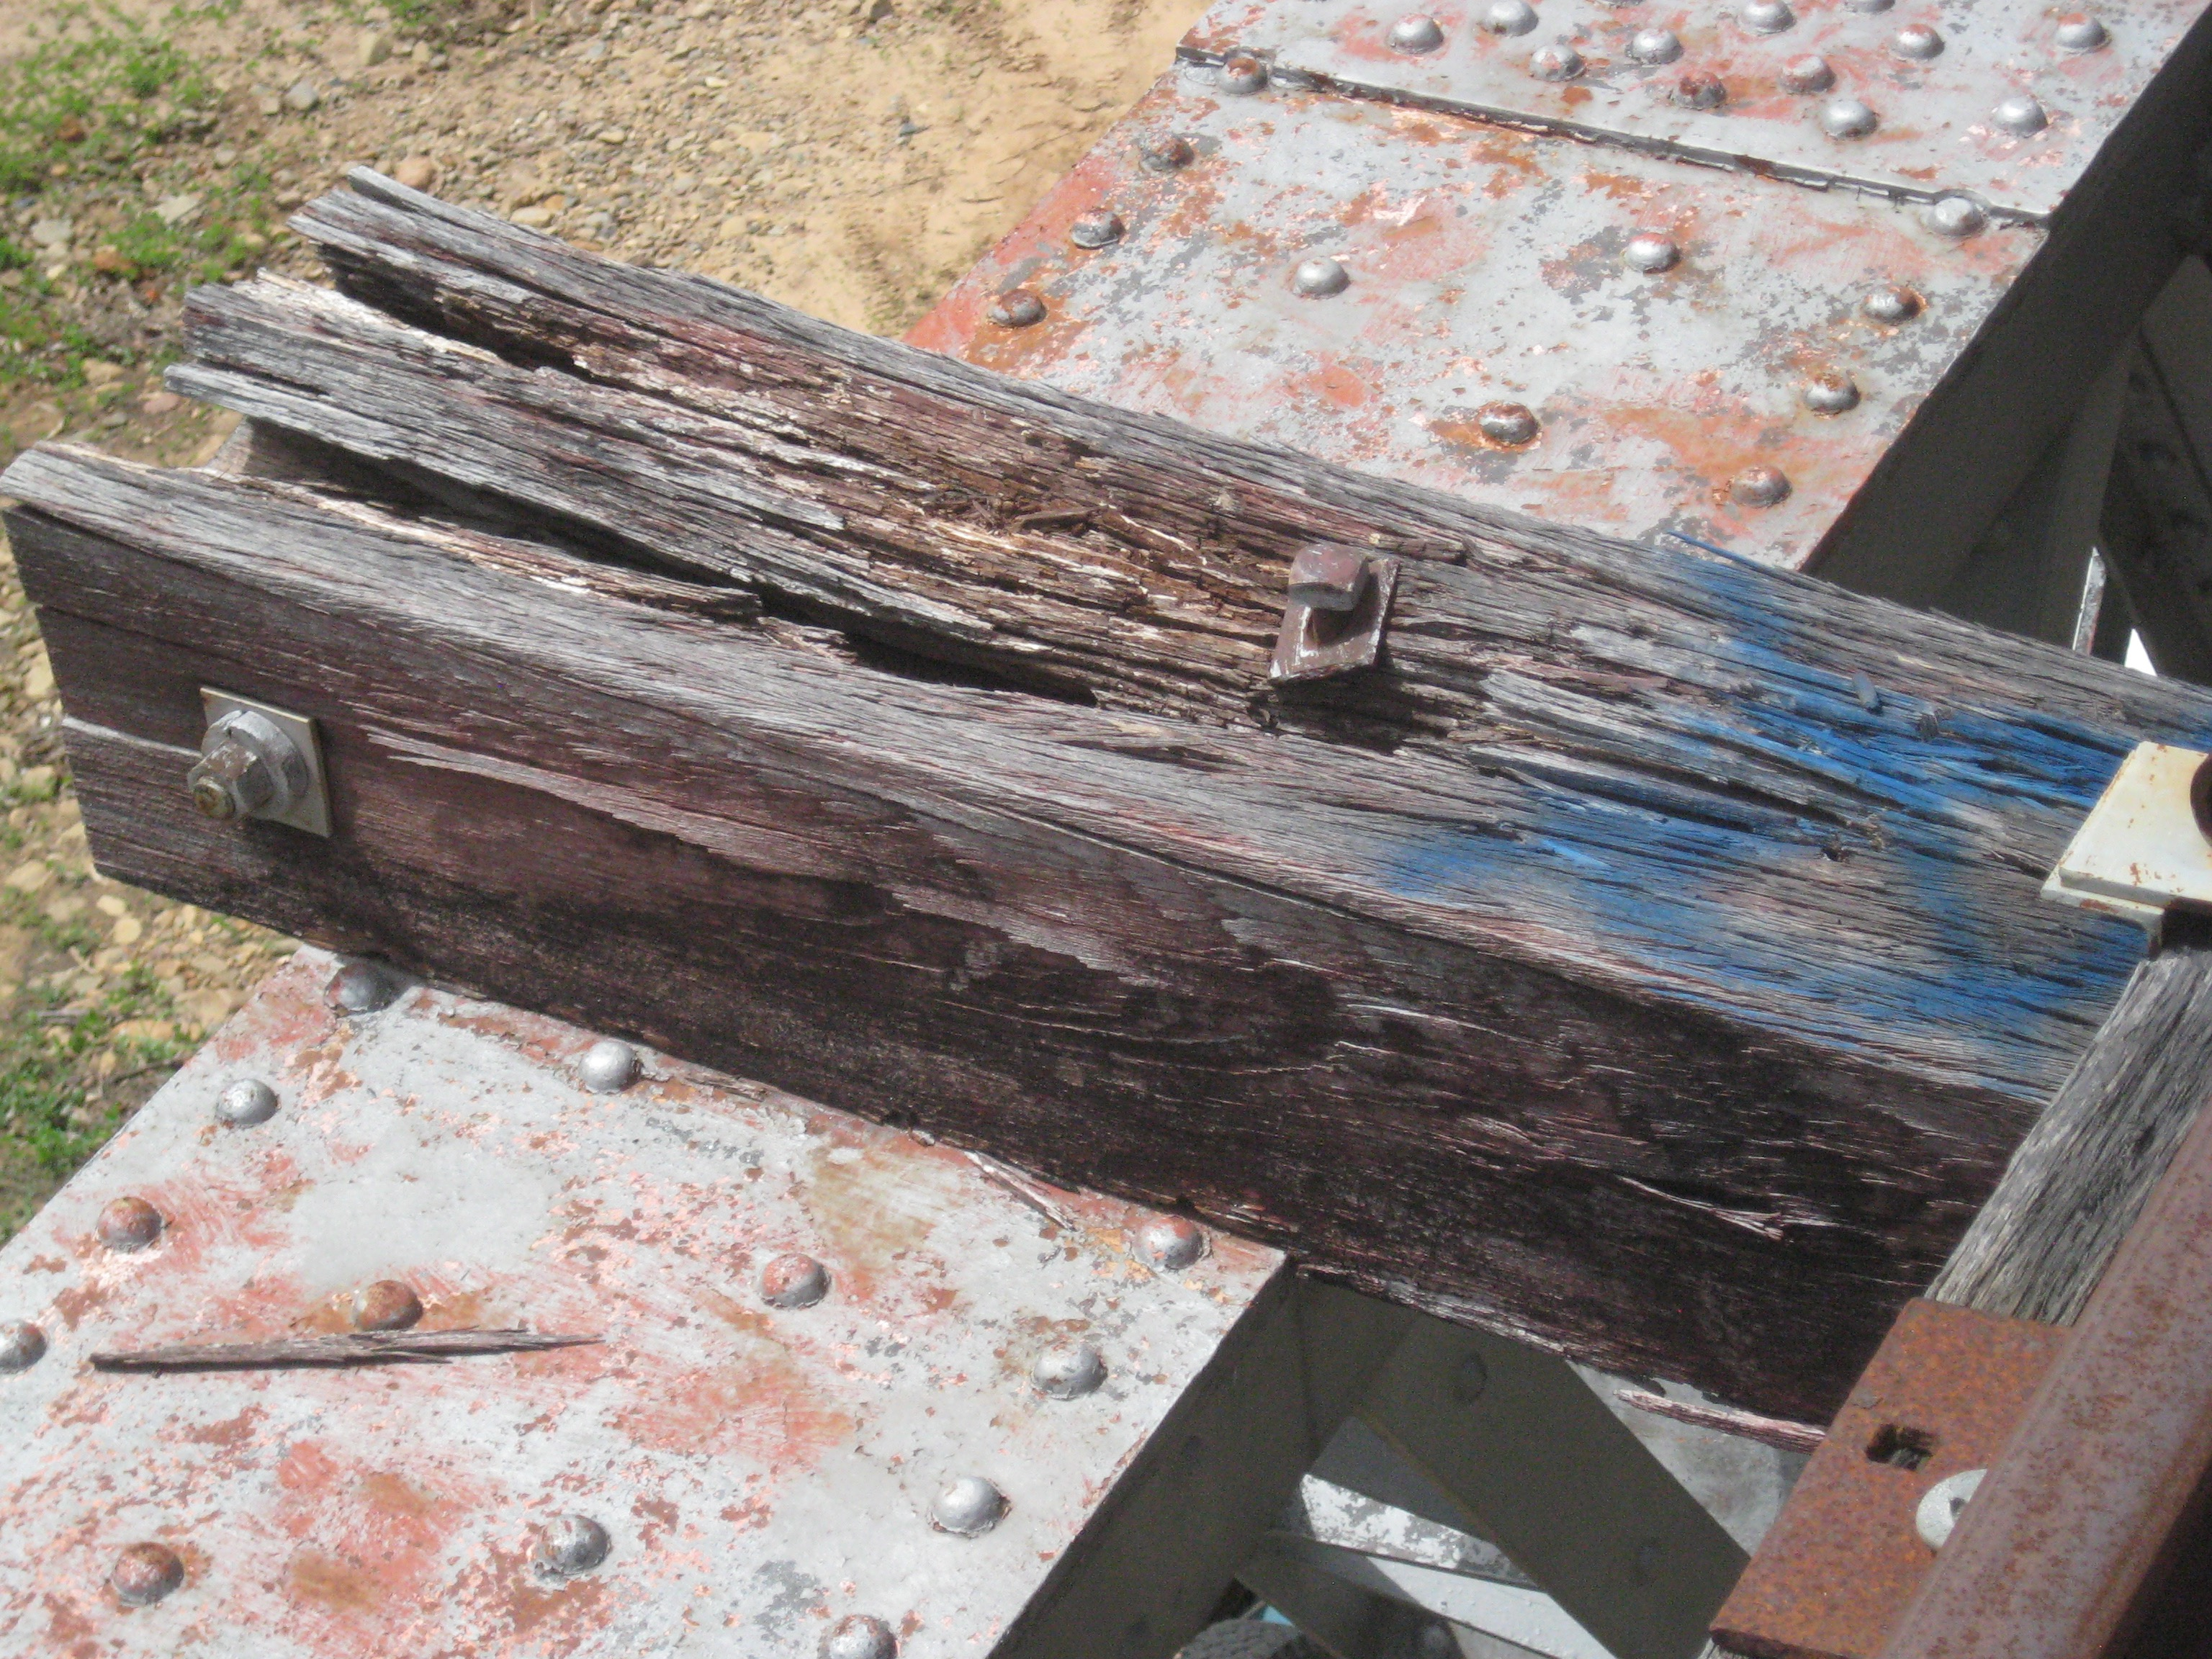
\includegraphics[scale=0.07]{Core_Rotting}
	 		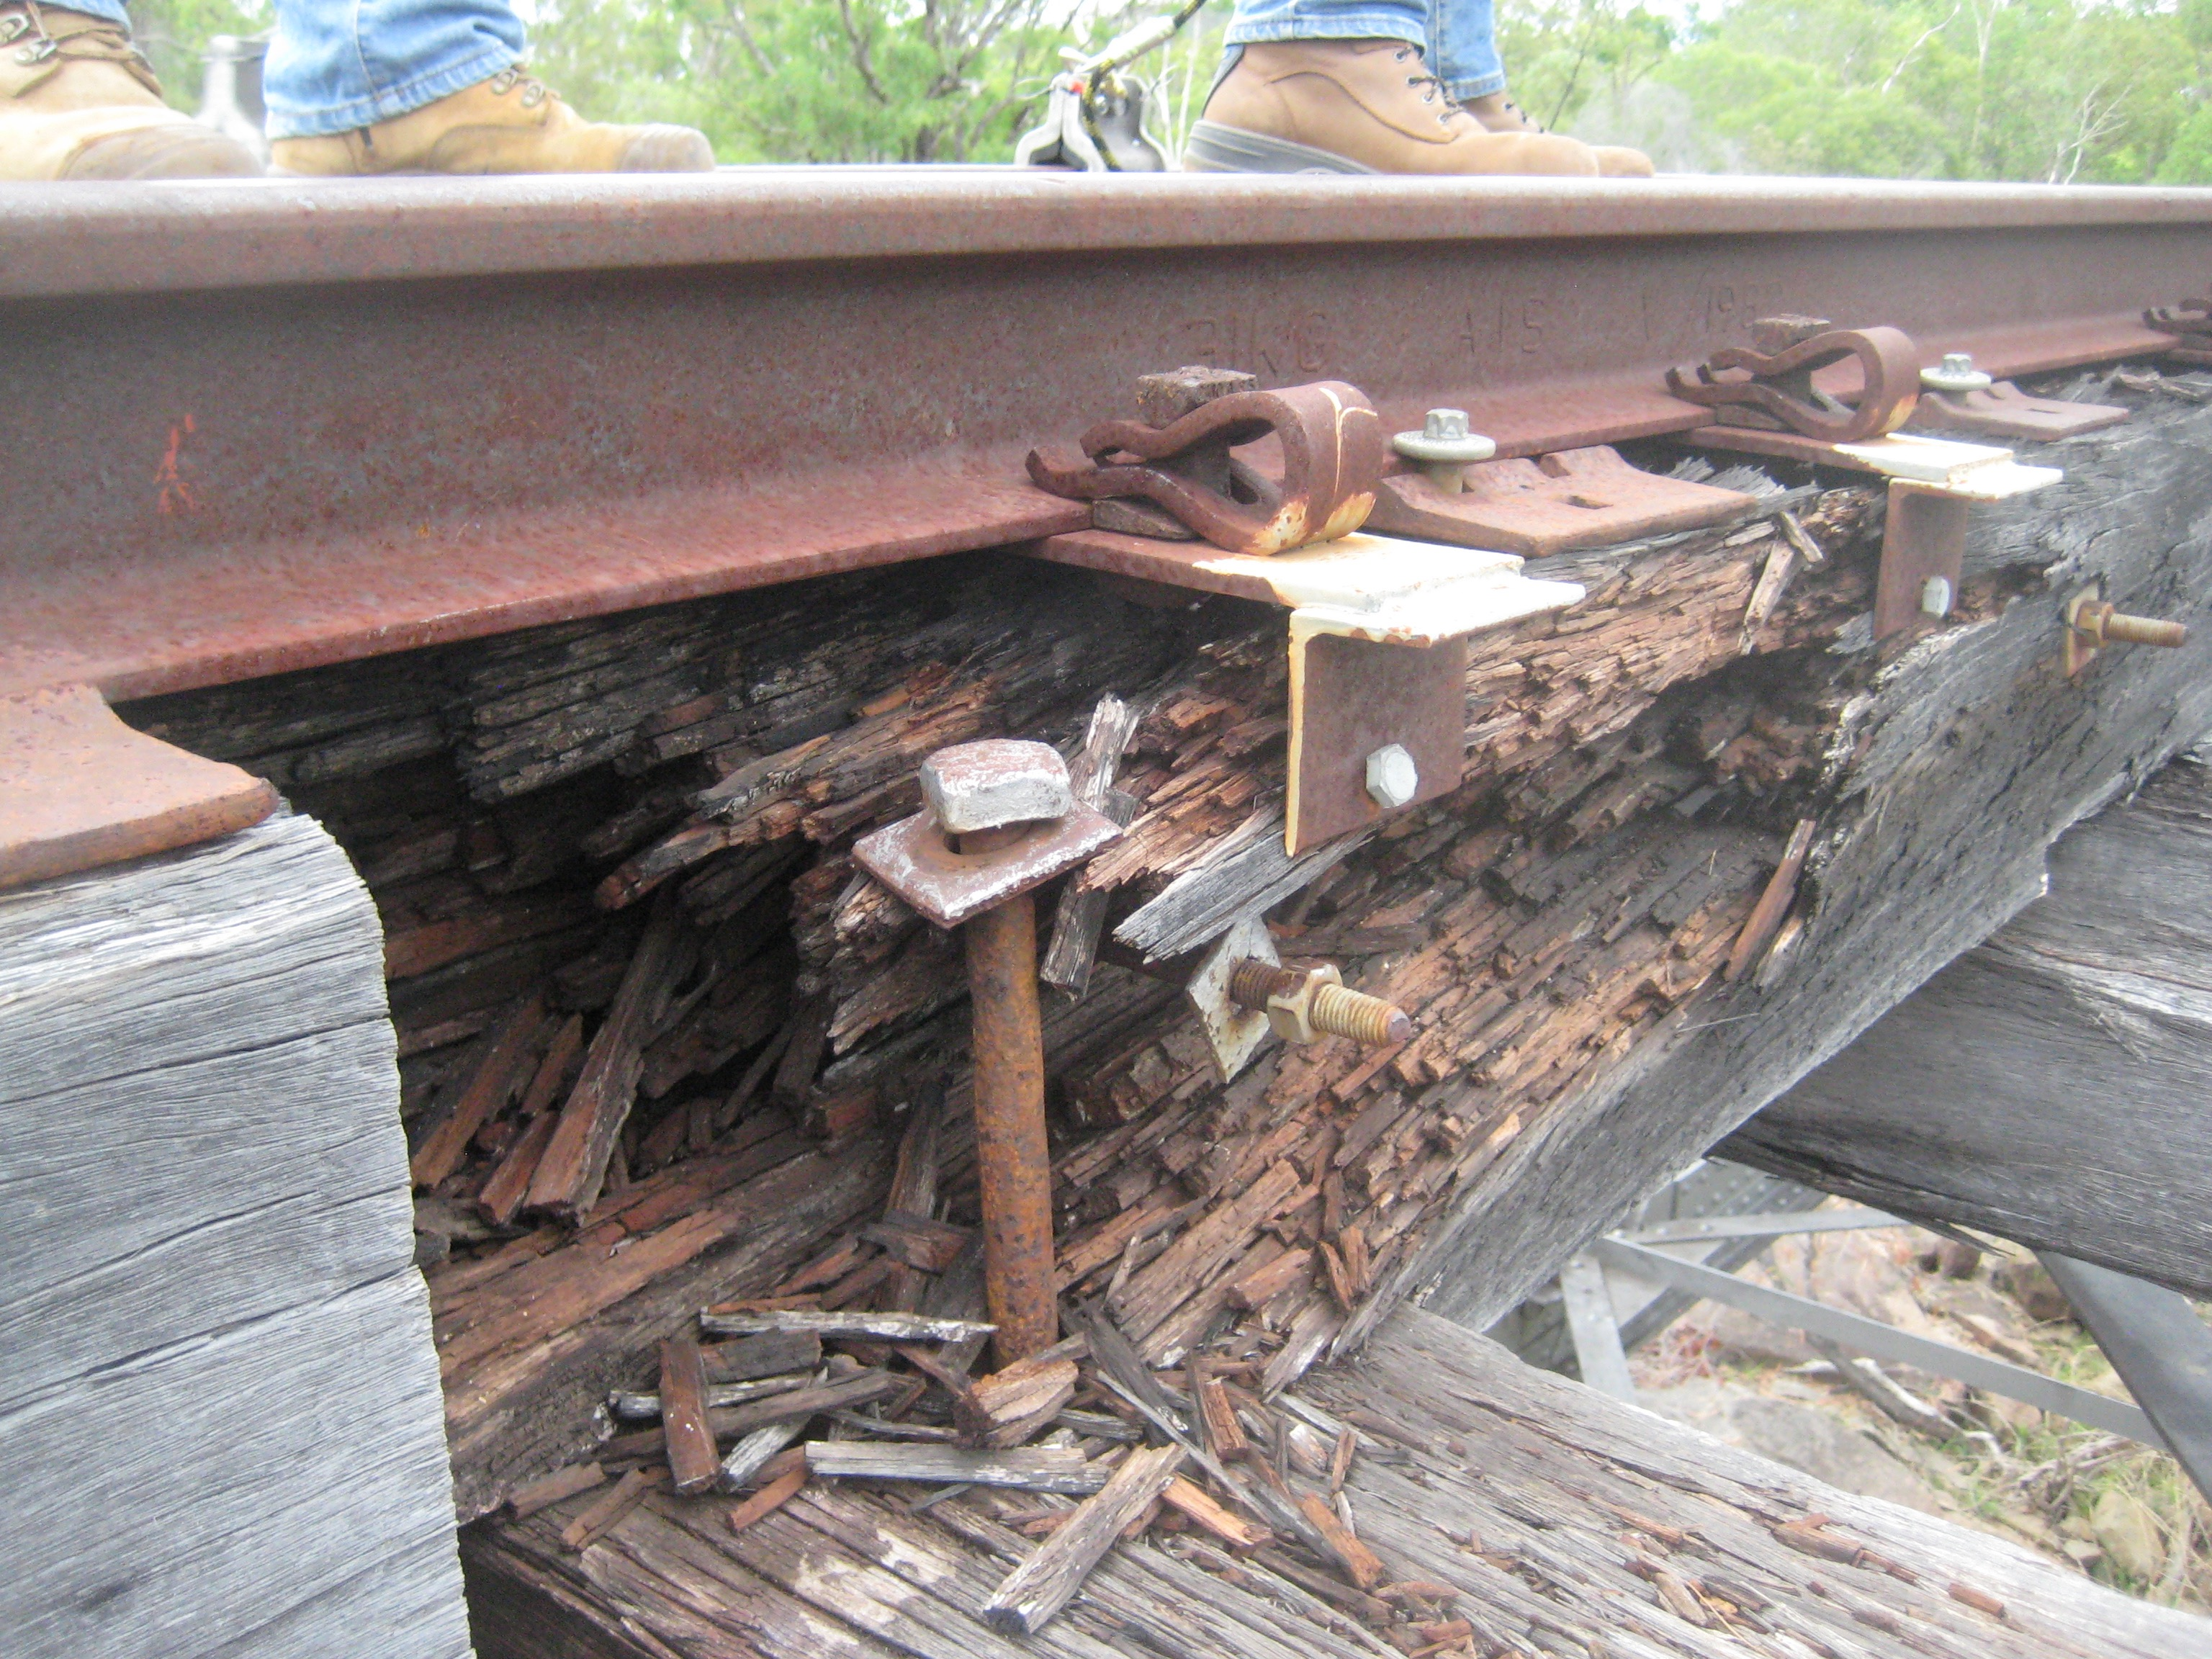
\includegraphics[scale=0.07]{Notch_Rotting}
	 		\caption{Core and Notch Rotting}
	 	    \label{fig:Rot}
	 	\end{figure} 
	
	\noindent
	Rot is decay caused by wood-destroying fungi which requires adequate moisture \cite{heckroodt_guide_2002}, heat and oxygen to prosper. This results in two different types of decay; brown rot and white rot. Brown rot is common in softwood where the fungi attacks only the cellulose creating a brown colour. However, white rot is more common in hardwood and is caused by the fungi attacking both the cellulose and lignin in the wood, creating a white colour. Rotting overall allows the rapid absorption of water and can be identified by a colour change or odor similar to anise or wintergreen\cite{white_bridge_1992}. Both weathering and rotting are effects of long-term exposure to the environment and can lead to a significant reduction in the strength of the member and potentially failure.
	
    \vspace*{\baselineskip}
	    
    \noindent
    \textbf{Insects}\par
    \noindent
    Timber is prone to two main types of insect attack; termite and lyctids. Termites require mois-ture, warm temperatures, access to their nest and usually ground contact to prosper. The most effective way to avoid termite damage is to use a timber species that is resistant to termites. Alternatively, preservative treated timber can be used or a physical or chemical barrier can be created between the timber ends and the nests \cite{_section_2008}.
	
	\vspace*{\baselineskip}
	
	\noindent
	Only the sapwood present in specific hardwoods are vulnerable to lyctids (or powder post beetles), softwoods are resistant to attack from these insects. Thus the use of softwoods or avoidance of the used of certain susceptible hardwoods will reduce the risk on lyctid attack \cite{_section_2008}.
	
	 \vspace*{\baselineskip}
	 
	\noindent
	Both these types of insects cause the same issues in timber; where they tunnel through the wooden members, causing large amounts of intricate bored out networks. This severely reduces the member strength and can eventually cause failure \cite{ryall_bridge_2001}.

	
    \vspace*{\baselineskip}
    
    \noindent
    \textbf{Cracking}
    
    \noindent
    Cracking usually occurs due to applied loads (dead and live) exceeding the strength capacities of the timber member and will eventually lead to failure. This defect can occur in any conditions and is purely dependent on the loads that are applied. However the presence of other capacity reducing defects can significantly increase the chances of cracking. The two types of cracks that occur are flexural and shear cracking \cite{_timber_2005}.
	
    \vspace*{\baselineskip}	
	
	\noindent
	Flexural cracks appear on the areas of a bridge that have high moments due to applied loads. The common location for flexural cracking are at the mid-span of the member, over the support and underneath any other permanent loads (dead loads). These areas are depicted in the Figure \ref{fig:Flex} \cite{_timber_2005}.  

 	\begin{figure}[h]
        \begin{center}
		 	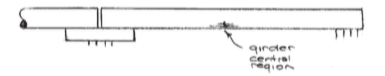
\includegraphics[scale=0.8]{Failure_Location_1}
	 		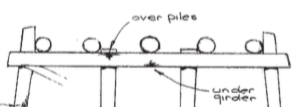
\includegraphics[scale=0.8]{Failure_Location_2}
        \end{center}
	 		\caption{Locations of Flexural Cracking or Crushing \cite{_timber_2005}}
	 		\label{fig:Flex}
	\end{figure}
\pagebreak

    \noindent
	Cracking due to flexure occurs in the tensile region or face of the member and can also result in the occurrence of crushing in the compression region. Hence, flexural cracking can be a combination of tensile and compressive failure \cite{thelandersson_timber_2003}. 

    \vspace*{\baselineskip}	
    
	\noindent
	Shear cracking is caused by the shear capacity of the timber being exceeded by applied loads, resulting in horizontal cracks propagating along the grain, as shown in Figure \ref{fig:Shear}. These cracks occur in high shear stress regions throughout the bridge such as over piles and at the ends of girders \cite{_timber_2005}. 
	
	\begin{figure}[h]
 		\begin{center}
 			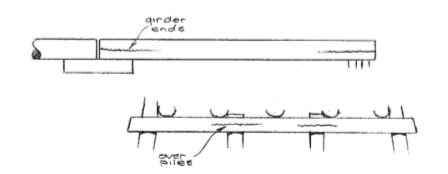
\includegraphics[scale=0.8]{Shear_Failure}
 		\end{center}
 		\caption{Locations of Shear Cracking \cite{_timber_2005}}
 		\label{fig:Shear}
 	\end{figure}
   \noindent 
   Both flexural and shear cracking on bridges is usually a result of bending which can cause forces in tension, compression and shear as well as moments \cite{ritter_timber_1990}. 

\subsection{Timber Properties}
    Timber is a very unique structural material and differs significantly from other man-made materials, such as steel or concrete \cite{plevris_frp-reinforced_1992}. This is due to its fibrous cell structure.
	
	\vspace*{\baselineskip}	
	
	 \noindent
	 The primary forms of failure in timber beams are tensile, shear and compressive failure. For timber, the stress-strain relationship is assumed to be uniaxial \cite{bazan_ultimate_1980,buchanan_combined_1986}, as shown in Figure \ref{fig:Stress-Strain}, where the negative region describes compression and positive region is in tension.
	 
	\begin{figure}[h]
  		\begin{center}
  			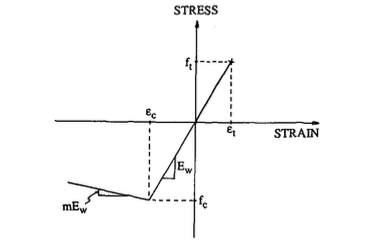
\includegraphics[scale=0.9]{Stress_Strain_Wood}
  		\end{center}
  		\caption{Standard Stress-Strain Diagram of Timber \cite{plevris_frp-reinforced_1992}}
  		\label{fig:Stress-Strain}
  	\end{figure}
	 
	 \noindent
	 The member fails in tension at a stress $f_{t}$, with a relating strain $\varepsilon_{t}$, and in compression fails at a stress $f_{c}$ and strain $\varepsilon_{c}$. The Young's modulus of the wood ($E_{w}$) is the gradient of the stress strain relationship. Beyond the compression-strain at failure ($\varepsilon_{c}$) the gradient and direction of the line changes by a constant ratio m of the Young's modulus \cite{plevris_frp-reinforced_1992,fiorelli_fiberglass-reinforced_2006}.
	 
     \vspace*{\baselineskip}	
	 
	 \noindent
	 Tensile failure is a brittle failure and is usually caused by long-term constant distributed loading. Longer members are more susceptible to tensile failure which occurs at the weakest point on the beam. Compressive failure is also caused by long-term loading and is a ductile failure \cite{thelandersson_timber_2003}. 
	 
     \vspace*{\baselineskip}
	 
   	\noindent
   	Modulus of rupture (MOR) is the maximum allowable stress a species of timber can withstand before its fibres rupture or break; which defines the bending strength \cite{markwardt_strength_1935}. It can be calculated from the maximum load the beam can carry ($F_{R}$) \cite{walker_primary_2013}  and is given by
   	
   	\begin{equation}
   	MOR = \dfrac{M}{Z} 
   	\end{equation}
   	
   	\begin{equation}
   	MOR \approx \dfrac{3 F_{R} l}{2bh^{2}} 
   	\end{equation}
   	
   	\noindent
   	where; \par
   	$ l $ = Span of the beam \par
   	$ b $ = Width of the beam \par
   	$ h $ = Height of the beam. \par
   	$ Z $ = Section modulus \par
   	 
   	\vspace*{\baselineskip}
   	
   	\noindent
   	 The modulus of elasticity (MOE) measures the flexibility or stiffness of timber and is determined through bending and deflection \cite{walker_primary_2013,agriculture_encyclopedia_2007}. The MOE in bending, also commonly denoted as $E_{b}$, can be determined from the load at the proportional limit ($F_{p}$) \cite{agriculture_encyclopedia_2007} and is given by
   	 
   	 \begin{equation}
  E_{b} \approx \dfrac{F_{p} l^{3}}{4 \Delta bh^{3}}
   	 \end{equation}
   		
   	\noindent
   	where; \par
   	$ \Delta $ = Deflection at midspan due to the load $F_{p}$.\par
   	 
   	\vspace*{\baselineskip}
	 
	\noindent 
	 The flexural ability and properties is predominately due to the aspect ratio of the wood. Aspect ratio is the defined as the ratio between the fibre length to the fibre thickness. Longer fibres result in superior mechanical properties compared to shorter fibres, thus a higher aspect ratio renders better flexural properties \cite{klyosov_wood-plastic_2007}.  
	 
	 \vspace*{\baselineskip}
	 
	 \noindent
	 The other form of failure in wood is shear failure, which is again caused by applied shear loads exceeding the shear capacity of the beam. The shear stress distribution of a standard rectangular beam can be seen in Figure \ref{fig:Shear-Stress}, and is of parabolic nature both along and perpendicular to the grain.
	 
	\begin{figure}[h]
		\begin{center}
			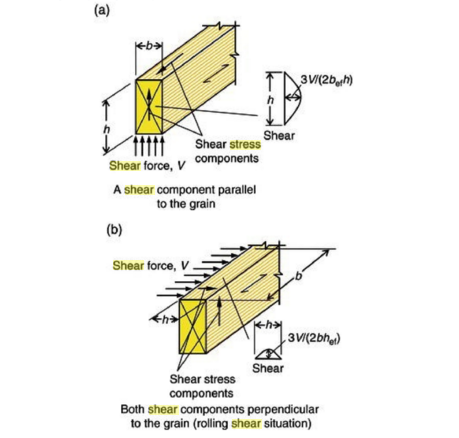
\includegraphics[scale=0.7]{Shear_Stress}
		\end{center}
		\caption{Shear Stress Distribution \cite{porteous_structural_2013}}
		\label{fig:Shear-Stress}
	\end{figure} 
	
	\pagebreak
	 
	 \noindent
	 The shear capacity of a timber species is a measure of the timber fibre's ability to withstand slippage. Shear capacity in timber is much greater across the grain than along the grain, where the fibres have to be broken, than along the grain where the fibres only need to be separated from each other \cite{walker_primary_2013}.
	
	
	\subsection{Australian Member Design}
	There are three common cross-sectional shapes of members in bridge construction; rectangular, circular and octagonal. The most commonly used is the rectangular section member, mainly for smaller scale constructions (e.g. frames, foot-bridges, etc.). However, for bridges requiring a large strength capacity, such as a rail bridge, the log can not be substantially reduced in size, as done to achieve rectangular cross-sections, thus the round and octagonal members are required. 
	
	
	\subsubsection{Rectangular Section}
	There are three standard Australian design codes that discuss design processes and equation for rectangular timber members; AS1720.1, AS4676 and AS4063. 

	 \vspace*{\baselineskip}
	 
	\noindent
	\textbf{Bending}\par
	% Discuss design aspects of a rectangular section member
	% Show equations and explain design process and necessary factors
	% Include all necessary tables and graphs
	
	\noindent
	The bending capacity ($M_{d}$) for an un-notched beam, with a rectangular section, is given in AS1720.1 as
	\begin{equation}
	\phi M_{d} = \phi k_{1} k_{4} k_{6} k_{9} k_{12} f'_{b} Z
	\end{equation}
	
	 where 
	 
	 $ \phi $ = Capacity Factor\par
	 
	 $ k_{1} $ = Duration of Load Factor\par
	 
	 $ k_{4} $ = Moisture Condition Factor\par
	 
	 $ k_{6} $ = Temperature Factor\par
	 
	 $ k_{9} $ = Strength Sharing Factor\par
	 
	 $ k_{12} $ = Slenderness Factor\par
	 
	 $ f'_{b} $ = Characteristic value for bending for section size
	 
	 $ Z $  = Section modulus of beam about bending axis.
	
	\vspace*{\baselineskip}
	
	\noindent
	All factors and the strength characteristic for bending can be determined from AS1720.1.
	
	\vspace*{\baselineskip}
	
	\noindent
	\textbf{Shear}\par
	
	\noindent
	The design capacity in shear of un-notched beams is described by AS1720.1 as
	\begin{equation}
	V_{d} = \phi k_{1} k_{4} k_{6} f'_{s} A_{s}
	\end{equation}
	
	\noindent
	where $\phi$, $k_{1}$, $k_{4}$, and $k_{6}$ are as determined for bending capacity design, \par
	
	$ f'_{s} $ = Characteristic value in shear\par
	
	$ A_{s} $ = Shear plane area.\par
	
	\vspace*{\baselineskip}
	
	\noindent
	and the characteristic value in shear can be found in AS1720.1. \par
	
	\vspace*{\baselineskip}
	
	\noindent
	Also when the beam is loaded about its major axis in bending, the shear plane area can be found from the breadth (b) and depth (d) using
	\begin{equation}
	A_{s} = \dfrac{2bd}{3}
	\end{equation}
	
	\subsubsection{Circular Section}
	The amount of information and research surrounding circular section members are minimal, and there are few design equations determined specifically for these members. 
	
	\vspace*{\baselineskip}
	
	\noindent
	\textbf{Bending}\par
	% Discuss design aspects of a circular section member
	% Show equations and explain design process and necessary factors
	% Include all necessary tables and graphs
	\noindent
    AS1720.1 uses the rectangular formula with additional factors to account for the change in section shape. This formula and additional factors are
	\begin{equation}
	\phi M = \phi k_{1} k_{4} k_{6} k_{9} k_{12} k_{20} k_{21} k_{22} f'_{b} Z
	\end{equation}

    \noindent
    where $\phi$, $k_{1}$, $k_{4}$, $k_{6}$, $k_{12}$ are as for working rectangular design and \par
    
    $ k_{20} $ = Immaturity Factor\par
    
    $ k_{21} $ = Shaving Factor\par
    
    $ k_{22} $ = Processing Factor.\par
	
	\vspace*{\baselineskip}
		
	\noindent
	\textbf{Shear}\par
	\noindent
	The design shear capacity given by AS1720.1 is again a modification of the rectangular design approach and is given by 
	
	\begin{equation}
	V_{d} = \phi k_{1} k_{4} k_{6} k_{20} f'_{s} A_{s}
	\end{equation}
	
	\noindent
	where the factors, $f'_{s}$ and $A_{s}$ are as specified in rectangular design, and $k_{20}$ takes into account the maturity of the material. The shear plane area for a round member is\par
	
	\begin{equation}
	A_{s} = \dfrac{3\pi d^{2}}{16}
	\end{equation}
	
	
	\noindent
	
	\subsubsection{Octagonal Section}
    Queensland Department of Transport and Main Roads (TMR) suggests that the design of such members for bending, is the same as for rectangular sections \cite{_timber_2005}. However there is very little information surrounding octagonal member design and no design methods determined specifically for this shape cross-section.


	\subsection{Notching}
	Notching or sniping is when the lower corner of a member is cut to make insertion easier, and to increase the stability of the member when sitting on a pier/abutment. One of the major issues faced with notches are they significantly reduce the load-carrying and shear capacities of timber beams. For these reasons, it is suggested that the use of notches be avoided in practice, however in some situations they cannot be \cite{jockwer_state---art_2013,jockwer_structural_2014}.
	
	\vspace*{\baselineskip}
	
	\noindent
    The reduction in the shear capacity of the beam causes a brittle failure and cracking to initiate from the corner of the notch, and propagate along the direction of the grain \cite{jockwer_state---art_2013,_timber_2005}. Figure \ref{fig:Notch_Crack} indicates the common behaviour of notch cracking.
    
       	\begin{figure}[h]
       		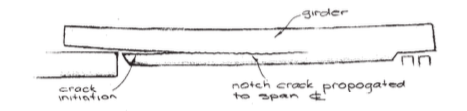
\includegraphics[scale=0.9]{Shear_Failure_Notching}
       		\caption{Notch Cracking \cite{_timber_2005}}
       		\label{fig:Notch_Crack}
       	\end{figure}
       
	\noindent
	To reduce the effects of capacity loss, TMR limit the section area loss from notching to be a maximum of 10\%. In cases where the notch is strengthened, a maximum allowable section loss can be up to 25\% \cite{_timber_2005}. As shown in Figure \ref{fig:Bending}, TMR also specifies that if there is less than 75\% of the original depth over the support, there is a high chance of failure to occur in bending. 
	
	       	\begin{figure}[h]
	       		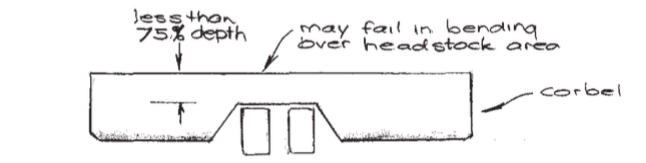
\includegraphics[scale=0.7]{Bending_Fail}
	       		\caption{Member failure in bending over support \cite{_timber_2005}}
	       		\label{fig:Bending}
	       	\end{figure}
	
	\pagebreak
	
	\noindent
	There are three different types of fracture modes of a notch in a timber member which are dictated by the forces/stresses present at the notch corner. Figure \ref{fig:Frac_Mode} depicts these modes.

	       	\begin{figure}[h]
	       		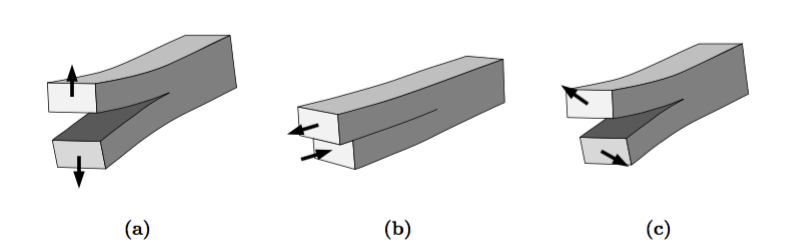
\includegraphics[scale=0.53]{Fracture_Modes}
	       		\caption{Fracture Modes (a) mode 1  (b) mode 2  (c) mode 3 \cite{jockwer_structural_2014}}
	       		\label{fig:Frac_Mode}
	       	\end{figure}
	
	\noindent
	Fracture mode 1 is when the crack propagating from the notch opens and is caused by tensile forces at the notch corner. Mode 2 is horizontal cracking/shearing, cause by shear forces acting along the grain at the notch corner. Lastly, mode 3 is a mixed mode fracture and is caused by a combination of both tension and shear forces \cite{jockwer_structural_2014}. 
	
	\subsubsection{Notch Types}
	There are four main types of notching, rectangular end notch, tapered end notch, rounded end notch and notch in span. The figure below shows the geometry of each type of notch.
	
	\begin{center}
		\begin{figure}[h]
			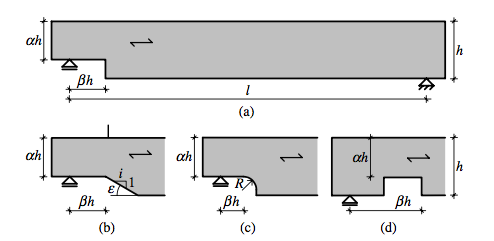
\includegraphics[scale=0.9]{Notch_Types}
			\caption{Notching Types; (a) rectangular end notch; (b) tapered end notch; (c) rounded end notch; (d) notch in span \cite{jockwer_state---art_2013}}
		\end{figure}
	\end{center}
	

	\noindent
	There is little information surrounding the exact effects of each type of notch on members. However, it is recommended by Australian Standard AS1720.1 that a tapered notch with a 1:4 gradient chamfer from the notch corner be used if notching is required. In theory, this particular tapered notch will increase the member's shear capacity by three times in comparison to a rectangular end notch\cite{_timber_2005}. 
	
	
	\subsubsection{Notch Design}	
	There are many different methods for designing notched members, based on significantly different concepts and, in most cases, obtaining varied results \cite{jockwer_structural_2014}. There are few methods in designing round end notches and notches within member spans, and most standards only design for a rectangular or tapered notch. However, the greatest limitation in notch design is all methods are based on rectangular section beams and do not account for circular or octagonal sections \cite{_timber_2005}. This is a major issue, as round and octagonal sections are preferred in timber bridges, due to their larger sections. 
	
	\vspace*{\baselineskip}
	
	\noindent
	\textbf{Australian Standards}\par
	\noindent
	The notched member design method used in AS1720.1 focuses on stress intensities and accounts for the effects of the maximum bending moment ($M^{*}$) and maximum shear force ($V^{*}$) occurring at the corner of the notch; where any negative values for bending moment or shear are neglected  \cite{jockwer_structural_2014}. AS1720.1 notch design equation is
	
	\begin{equation}
    \dfrac{6M^*}{bd_n^2} + \dfrac{6V^*}{bd_n} \leq \phi g_{40} k_1 k_4 k_6 k_{12} f'_{sj}
    \label{eq:Aus}
	\end{equation}
	
	\noindent
	where \par
	$ f'_{sj} $ = Shear strength\par
	$ g_{40} $ = Notch coefficient.\par
	
	\vspace*{\baselineskip}
	
	\noindent
	The k-factors and $\phi$ are purely dependent on location, use and specific timber characteristics, and are found as per usual design methods in AS1720.1. The other variables used in equation \ref{eq:Aus} are depicted in Figure \ref{fig:figure2}.
	
	\begin{center}
		\begin{figure}[h]
			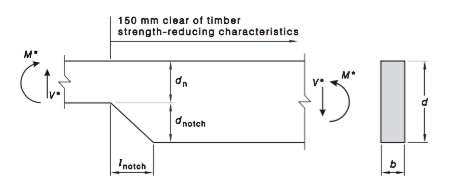
\includegraphics[scale=0.9]{Notching.png}
			\caption{Notation for Notch}
			\label{fig:figure2}
		\end{figure}
	\end{center}
	
	\pagebreak
	
	\noindent
	The notch coefficient g40 depends on the taper and height of the notch and can be found according to Table \ref{tab:g40}.
	
	\begin{center}
		\captionof{table}{Notch Coefficient}
		\label{tab:g40}
		\begin{tabularx}{\textwidth}{>{\centering}X|>{\centering}X|>{\centering}X} 
			\hline \hline
			\multirow{2}{*}{Notch Angle Slope} & \multicolumn{2}{c}{$g_{40}$} \\
			\cline{2-3}
			
			&$d_{notch} \geq 0.1d$ & $d_{notch} < 0.1d$ \tabularnewline [0.5ex] 
			\hline
			$l_{notch}/d_{notch}=0$ & $9.0/d^{0.45}$ & $3.2/d^{0.45}_{notch}$ \tabularnewline [0.5ex]
			\hline
			$l_{notch}/d_{notch}=2$ & $9.0/d^{0.33}$ & $4.2/d^{0.33}_{notch}$ \tabularnewline [0.5ex]
			\hline
			$l_{notch}/d_{notch}=4$ & $9.0/d^{0.24}$ & $5.2/d^{0.24}_{notch}$ \tabularnewline [0.5ex]
			\hline \hline
		\end{tabularx}
	\end{center}
	
	\vspace*{\baselineskip}
	
    \noindent
	AS1720.1 specifies that for this design method, no strength-reducing characteristics, such as knots, are allowed within 150mm from the notch corner.
	\vspace*{\baselineskip}
		
	\noindent
	Australian design method is based on LEFM, which is basic fracture mechanic concepts under the assumptions that the material is linearly elastic. However this assumption is not ideal for timber, as it's elastic properties are considered orthotropic. 
	
	\vspace*{\baselineskip}
	
	\noindent 	
	\textbf{Fracture Mechanics}\par 	 	
	\noindent 	
	The AS1720.1 notched member design method considers only the effect of stress intensities and does not take into account fracture mechanics. In 1988, Gustafsson proposed an equation to design for strength of the notch, based on fracture energy \cite{jockwer_state---art_2013,gustafsson_study_1988}.  	 \begin{equation} 
	\dfrac{V_{f}}{b\alpha d} = \dfrac{\sqrt{\frac{G_{c}}{d}}}{\sqrt{0.6\frac{(\alpha-\alpha^{2})}{G_{xy}}}+\beta\sqrt{6\frac{(1/\alpha-\alpha^2)}{E_{x}}}} \end{equation} 		 		 		
	\noindent 		
	Where; \par 	
	$ V_{f} $ - Shear force at fracture of notch\par 	
	$G_{xy}$ - Shear modulus\par  	
	$ E_{x} $ - Modulus of elasticity in beam direction, parallel to the grain\par 	
	$ d $ - depth of the member\par  	
	$ G_{c} $ - Fracture energy\par  	
	$ \beta $, 
	$ \alpha $ and h are depicted in the figure below. \par 		 	
	\vspace*{\baselineskip} 	 	
	\noindent 	This equation was established for a beam notched at both ends, and in accordance with the characteristics shown in the figure \ref{fig:Gust}. The actions due to the moment and shear, along with the effect from elastic clamping, results in a deflection, which is the basis of this fracture energy approach. Gustafsson derived this deflection, also considering lower bending stiffness of the cross-section at the junction of the notched part of the beam, and assumed its proportionality to the moment acting at the notch corner \cite{jockwer_state---art_2013}. Clamping was also incorporated with a factor, which was conservatively chosen as $1/\alpha^{3}$ \cite{gustafsson_study_1988}.   
		 	 		
		\begin{figure}[h] 			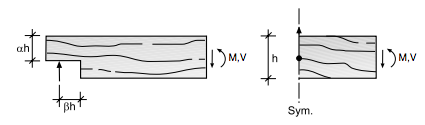
\includegraphics[scale=0.9]{Geom_notched_beam_dowl} 			\caption{Geometry of notched beam and dowel joint \cite{serrano_fracture_2007}} 	
		\label{fig:Gust}	
		\end{figure} 	
	 		 	
	\noindent 	
	The fracture energy for a notched member can be found using the following equation \cite{serrano_fracture_2007}.  	 	
	\begin{equation} 		
	G_{c} = \dfrac{1}{2}(P_{f}^{2}/B) \dfrac{dC(a)}{da}  	\end{equation} 	 	
	Where;\par 	
	C - denotes the compliance of the structure\par 	
	da - extension of the length of the crack\par 	
	$P_{f}$ - magnitude of load that start propagation of the crack\par 	
	B - width of the fracture area (i.e. $B = dA/da$) 
	   
	 \vspace*{\baselineskip} 	 	
	 
	 \noindent 
	 Similar notch strength equations have been derived (Smith et al. 1996), with a defining difference of the clamping effect. Smith et al proposed a notch strength relationship from the same fracture mechanic concepts, but taking a clamping factor of $1/\alpha^{2}$. It has been found through comparison, that the prediction of the notch strength proposed by Gustafsson was more conservative and accurate than Smith et al. which has given results exceeding the notches capacity \cite{jockwer_state---art_2013}.   	
	 
	 \vspace*{\baselineskip} 	 	
	 
	 \noindent 	This approach is used as a verification of the shear stress in the notch cross-section and has become a basis for design methods in European and Canadian design codes.
	
	\vspace*{\baselineskip}
	
	\noindent
	\textbf{Eurocode 5 Approach}\par
	
	\noindent
	The European timber structure design code (Eurocode 5) is based on studies of notch fracture mechanics and specifies the following equation for notch design as
	 
	\begin{equation}
	\tau_{d} = 1.5\dfrac{V}{b h_{ef}} \leq k_{v} f_{v,d} 
	\end{equation}
     
     where\par
     $ \tau_{d} $ = Shear stress \par
     $ V $ = Shear force \par
     $ h_{ef} $ = Depth above notch \par    
     
     \vspace*{\baselineskip} 
     
     \noindent
     The shear strength, $ f_{v,d} $, can be found using
     
   	\begin{equation}
   	f_{v,d} = \dfrac{k_{mod} f_{v,k}}{\gamma M} 
   	\end{equation} 
     
     \noindent
     where $f_{v,k}$ is the characteristic shear strength, $k_{mod}$ is a strength modification factor and $\gamma M$ is a material modification factor, all of which can be found in Eurocode 5 \cite{_eurocode_1995}.
     
     \vspace*{\baselineskip} 
     
     \noindent
     The notch factor $k_{v}$ is derived from Gustafsson's 1988 equation \cite{gustafsson_study_1988}, as well as modifications to account for the taper of the notch ($i$) established by Riberholt \cite{riberholt_timber_1991} and is given by
     
     \begin{equation}
     k_{v} = min
     \begin{cases}
	 1  \\ 
	 \frac{k_{n}(1+\frac{1.1i^{1.5}}{\sqrt{h}})}{\sqrt{h}(\sqrt{\alpha(1-\alpha)} + 0.8\frac{x}{h} (\sqrt{\frac{1}{\alpha}-\alpha^{2}})}
    \end{cases}
    \end{equation}
	
	\vspace*{\baselineskip}
	
	\noindent
	Overall, the notch factor considers the notch taper $i$, material constant $k_{n}$, ratio of depth above notch to total depth $\alpha$, the distance to the support $x$, and the total depth of the beam h \cite{_timber_2005,jockwer_structural_2014}.
	
	\vspace*{\baselineskip} 
	
	\noindent
	\textbf{CSA O.86 Approach}\par
	
	\noindent
     The Canadian design code (CSA 0.86:2014) is also based on fracture mechanics and thus has a similar design concept to Eurocode 5 \cite{jockwer_structural_2014}. However, the design is based around the verification of the resistance of the notch ($F_{r}$) instead of the stresses, which is calculated by
     
	\begin{equation}
	F_{r} = \Phi F_{f} A K_{N} 
	\end{equation}     
     
     where\par
     $ \Phi $ = Resistance factor (given as 0.9) \par
     $ A $ = Cross-sectional area
     
     \vspace*{\baselineskip}
     
     \noindent
     $F_{f}$ can be calculated from $f_{f}$ and Equation \ref{eq:Ff} \cite{_csa_2014,_errata:_2013}.
     
   	\begin{equation}
   	F_{f} = f_{f} K_{D} K_{H} K_{Stp} K_{T}
   	\label{eq:Ff} 
   	\end{equation}  
     
     \noindent
     Where $f_{f}$ is given as 0.5MPa for sawn lumber and the condition ($K$) values can be found in CSA O.86.
 
     \vspace*{\baselineskip}
    
     \noindent    
     $K_{N}$ is the notch factor and can be found using Equation \ref{eq:kn} \cite{jockwer_structural_2014,_csa_2014}. The notch factor is based on studies by Smith and Springer, and takes into account the depth of the beam ($d$), notch ratio $\alpha$ and notch length ratio $\eta$ \cite{smith_consideration_1993}.
     
	\begin{equation}
	K_{N} = \bigg\{0.006d \bigg[1.6 \bigg(\dfrac{1}{\alpha}-1 \bigg)+\eta^{2} \bigg(\dfrac{1}{\alpha^{3}}-1\bigg) \bigg] \bigg\}^{1/2} 
	\label{eq:kn}
	\end{equation} 
    
    where\par
    $ d $ = Total depth of member \par
    $ d_{n} $ = Depth of notch \par
    $ e $ = Length of notch from centre of support \par
    $\alpha = 1 - d_{n}/d$ \par
    $\eta = e/d$ \par
 
    \vspace*{\baselineskip}

    \noindent
    To satisfy CSA O.86 design requirements, the design shear load ($Q_{f}$) must be less than the notch resistance load ($F_{r}$) \cite{_csa_2014,_errata:_2013}.   

\subsection{Timber Strengthening}
There are many methods used to strengthen timber structures \cite{plevris_frp-reinforced_1992}. These techniques are based around combining various different forms of reinforcement to the members. Basic forms of reinforcement have been utilised such as steel bars, steel and aluminium plates and externally bonded plywood. There have also been some slightly more complex strengthening efforts. In 1965, Peterson \cite{leicester_size_1969} attempted to prestress glulam timber beams using stressed steel plates. This was achieved by fixing the steel plates to the tension side of the glulam beam using epoxy. Others include pre-stressing glulam using cable and strengthening using steel tension bearing embedded wire. 

\vspace*{\baselineskip}

\noindent
A popular form of reinforcement of timber beams is the use of fibre reinforced polymers (FRP) composites. This form of reinforcement is unique because of its ability to improve structural strength, stiffness and ductility characteristics, maintaining a very light weight \cite{plevris_frp-reinforced_1992}. Although many methods of timber strengthening has been tested, there are few recorded efforts in testing strengthened notched timber members. 


\subsubsection{Strengthening of Notched Beams}
Due to the abrupt change in the section area from a notch, high stresses are concentrated at the corner of the notch and can develop cracks. Extensions of these cracks can lead to failure and thus reinforcing notches is required to reduce the risk of cracking \cite{jockwer_structural_2014}. Notches can be reinforced either internally (Figure \ref{fig:Internal}) or externally (Figure \ref{fig:External}). Internal reinforcements are usually screwed/glued in rods and fully threaded screws. It should be noted that the screws and rods must be tight fitting to reduce the impact of shrinkage and water penetrating the hole\cite{jockwer_structural_2014,fawwaz_structural_2012}. 

	\begin{center}
		\begin{figure}[h]
			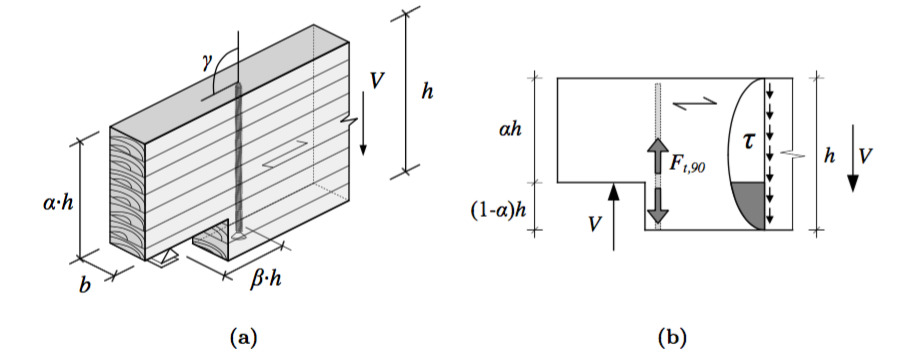
\includegraphics[scale=0.5]{Notch_Screw}
			\caption{(a) Parameters of internal reinforcement  (b) The theoretical portion of the shear stress taken by the reinforcement  \cite{jockwer_structural_2014}}
			\label{fig:Internal}
		\end{figure}
	\end{center}
	
\vspace*{\baselineskip}
	
\noindent
Bolts have been used as a standard notch strengthening method by TMR and are commonly M24 galvanised bolts, inserted perpendicular to the grain and extending through the full depth of the member. A 3mm thick plate is used at either end of the bolt to reduce cracking and pull out effects. The bolts are threaded at both ends and held on by nuts as shown in Figure \ref{fig:Internal2} \cite{_timber_2005}

	\begin{center}
		\begin{figure}[h]
			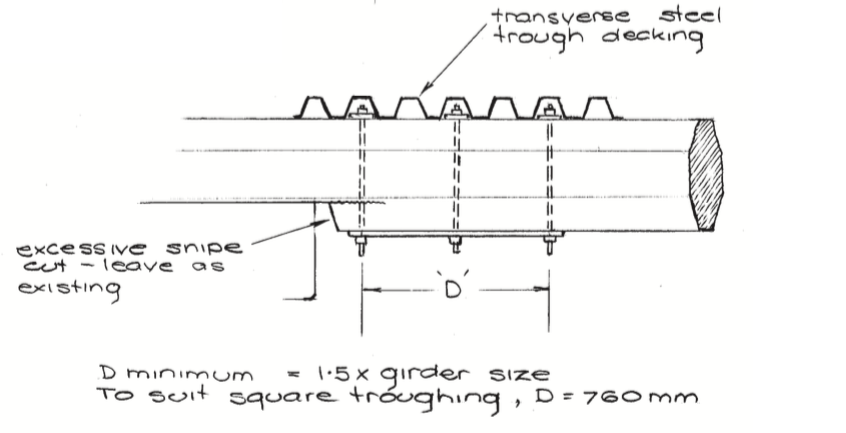
\includegraphics[scale=0.5]{Bolt_Layout}
			\caption{TMR Standard Bolt Layout \cite{_timber_2005}}
			\label{fig:Internal2}
		\end{figure}
	\end{center}
	

\noindent
External notch reinforcement methods are commonly adhered plywood, LVL or lamellas of solid timber and metal plate fasteners \cite{jockwer_structural_2014,fawwaz_structural_2012}. These are used to increase the strength capacities of the notch corner and reduce the risk of cracking. 

\vspace*{\baselineskip}

\noindent
Steel straps have also been used by TMR to reduce notching effects on piles, as seen in Figure \ref{fig:External}. However this method has not been used to reinforce girders. Essentially, a strap works similarly to a plate or wrap, where is compacts the notch corner and reduces the effects from notch cracking. 

	\begin{figure}[h]
		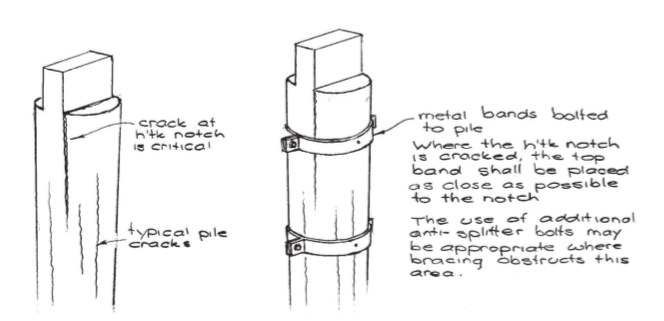
\includegraphics[scale=0.6]{Piles}
		\caption{Straps on Piles \cite{_timber_2005}}
		\label{fig:External}
	\end{figure} 
	\pagebreak

\noindent
In both external and internal reinforcement methods, studies have been undertaken where the material has been replaced with fibre reinforcement polymers (FRP) \cite{jockwer_structural_2014}. However these studies were carried out on rectangular sectioned beams and there is no recorded studies on the effects of notch reinforcement on circular members. 

\subsection{Analysis and Modelling}
For analysis and modelling purposes, timber can be assumed to have orthotropic properties in the longitudinal, tangential and radial directions \cite{kim_modeling_2010}. These directions are shown in Figure \ref{fig:Axes} with relation to the cross-sectional grain direction, where $L$ refers to longitudinal, $R$ to radial and $T$ tangential. This will assist in developing accurate models using finite element analysis (FEA) of a three-dimensional member. 

\begin{figure}[h]
	\begin{center}
		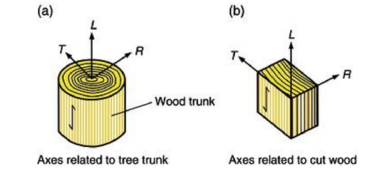
\includegraphics[scale=0.9]{Wood_Axes}
	\end{center}
 	\caption{Wood Axes \cite{porteous_structural_2013}}
 	\label{fig:Axes}
\end{figure}

\vspace*{\baselineskip}
\pagebreak

\section{Material and Methodology}
Notches are widely used throughout timber bridge construction as a method of seating over other members or piers. Due to the section loss caused by notching, horizontal splitting commonly occurs along the grain, which may result in failure. This is caused by high stresses occurring in the notch corners, particularly in shear, combined with a loss of member capacity due to the reduced area. Although there are design methods for notching, they differ between codes and are based on rectangular sections. This is a major issue as members commonly used in timber bridges are of circular section. To achieve a better understanding of notch behaviour, current design methods and how to improve notch strengths in circular members, the following experiments and numerical testing were undertaken. 

	\begin{enumerate}
		\item Carry out small scale tests on rectangular and round members to determine the critical notch angle for each profile
		\item Develop models of timber members on ANSYS to implement and calibrate finite element analysis 
	\end{enumerate}

\subsection{Test Set-up}
A three point loading set-up was used for all member testing throughout the experiments. The set up consisted of a centrally loaded, simply supported beam. Modelling carried out using ANSYS suggested that this location for loading would give the most critical effects and reduce any failure due to crushing over the notch. Steel plates with dimensions 5mm x 40mm x 60mm were used in conjunction with the supports to distribute the load onto to beam. All timber used will be of the same species and dimensions. The notches for all specimens have a maximum area loss of 30\% as specified by Australian standards. The tests will be carried out for both rectangular and circular section members and the moment of inertia and section modulus for both types of beams will be assumed to approximately constant. This will allow comparison in design methods and results. 

\vspace*{\baselineskip}

\noindent
The dimensions of the rectangular members that were tested in the first experiment were 60mm x 100mm x 800mm. Allowing for the 30\% maximum depth loss, the notch were be either back sawn to a depth of 30mm. The test set-up for the rectangular experiments can be seen in Figure \ref{fig:rect}.

 \begin{figure}[h]
 	\begin{center}
 		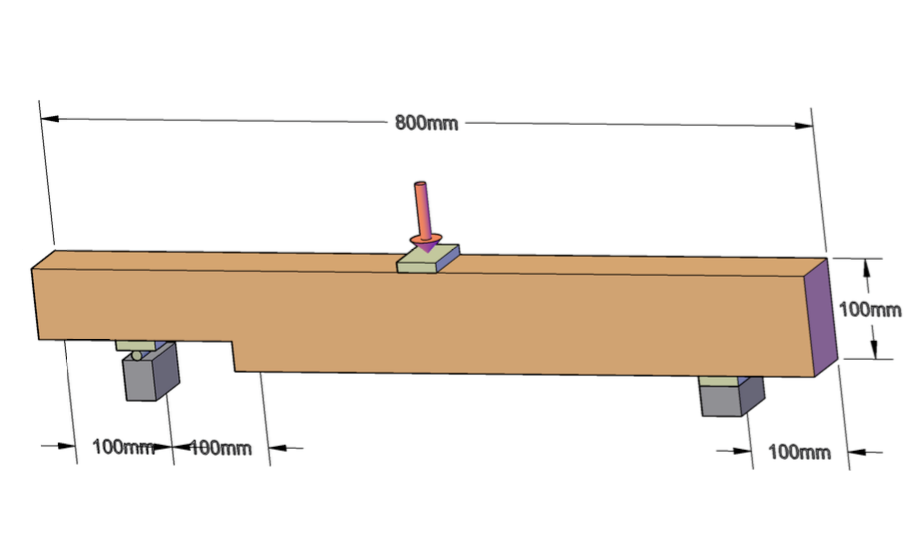
\includegraphics[scale=0.35]{Rectangular_Setup}
 	\end{center}
 	\caption{Rectangular Member Test Set-Up}
 	\label{fig:rect}
 \end{figure}

\pagebreak

\noindent
A 5mm x 40mm x 60mm steel plate was also placed at the centre of the beam and under the point load to distribute the load.

\vspace*{\baselineskip}

\noindent
The round members used for the experiments were 800mm in length with a 100mm diameter. To maintain a similar moment of inertia with the rectangular member, the notch was be cut to a depth of 25mm, which also stays within TMR's maximum limitations of 25\% depth loss. These members will be sawn so their grain profile will be radial and originating from the centre. This set-up can be seen in Figure \ref{fig:round}.


 \begin{figure}[h]
 	\begin{center}
 		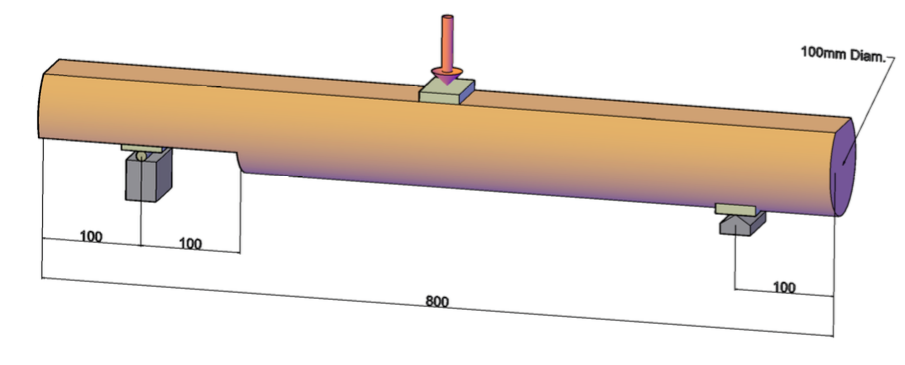
\includegraphics[scale=0.35]{Circular_Setup}
 	\end{center}
 		\caption{Round Member Test Set-Up}
 		\label{fig:round}
 \end{figure}
\pagebreak

\noindent
A rounded 5mm thick by 40mm wide metal plate was made, curving half of the members circumference, with a 3mm x 40mm x 300mm long, straight pieced of metal welded to one side to support the LVDT. 

\vspace*{\baselineskip}

\noindent
All tests were completed in the James Cook University structural engineering lab, using an Avery MTS to simulate three point loading with a controlled load rate. A load cell was also used in conjunction with the Avery to determine the load applied. 

\vspace*{\baselineskip}

\noindent
 The locations for the expected maximum loading effects on the beam will be determined using ANSYS modelling and FLA-2-11-3L strain gauges will be used for all tests to measure strains in these locations. An LVDT will also be used to measure the deflection below the applied load/notch corner. To collect all the data from the strain gauges, LVDT and load cell, a CR3000 Campbell?s scientific data logger will be used.

 \begin{figure}[h]
 	\begin{center}
 		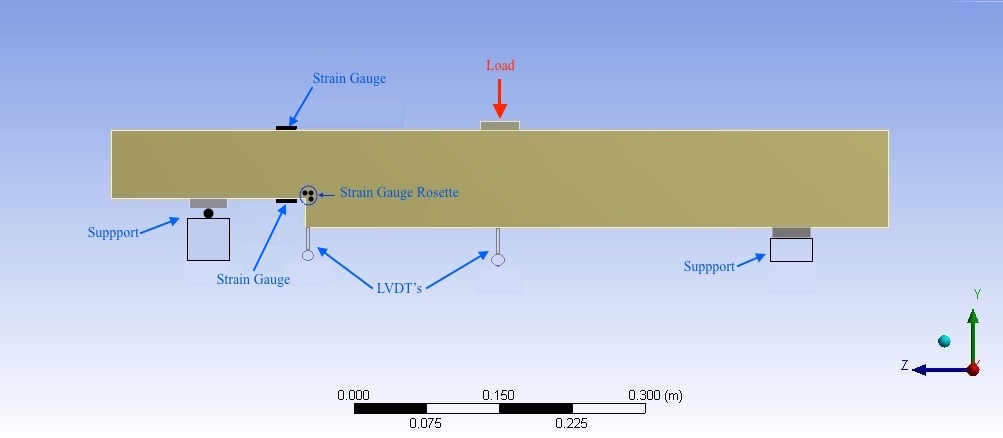
\includegraphics[scale=0.4]{Gauge_Set_up}
 	\end{center}
 	\caption{Strain Gauge and LVDT Layout}
 	\label{fig:Gauge}
 \end{figure}

\noindent
As shown in Figure \ref{fig:Gauge}, strain gauge rosettes will be placed at the notch corner as analysis has shown it endure high levels of strain. Strain gauges will also be placed on the tension and compression faces, as close as possible to the notch corner, to determine a strain and stress profile. 

\subsubsection{Altering Notch Angles of Small Scale Members}
Two notch types will be tested in this experiment; a rectangular end notch and a tapered end notch with slopes of 1:2 and 1:4. The strains surrounding the notch and failure type will be observed to determine the critical notch angle. 

\begin{figure}[h]
	\begin{center}
		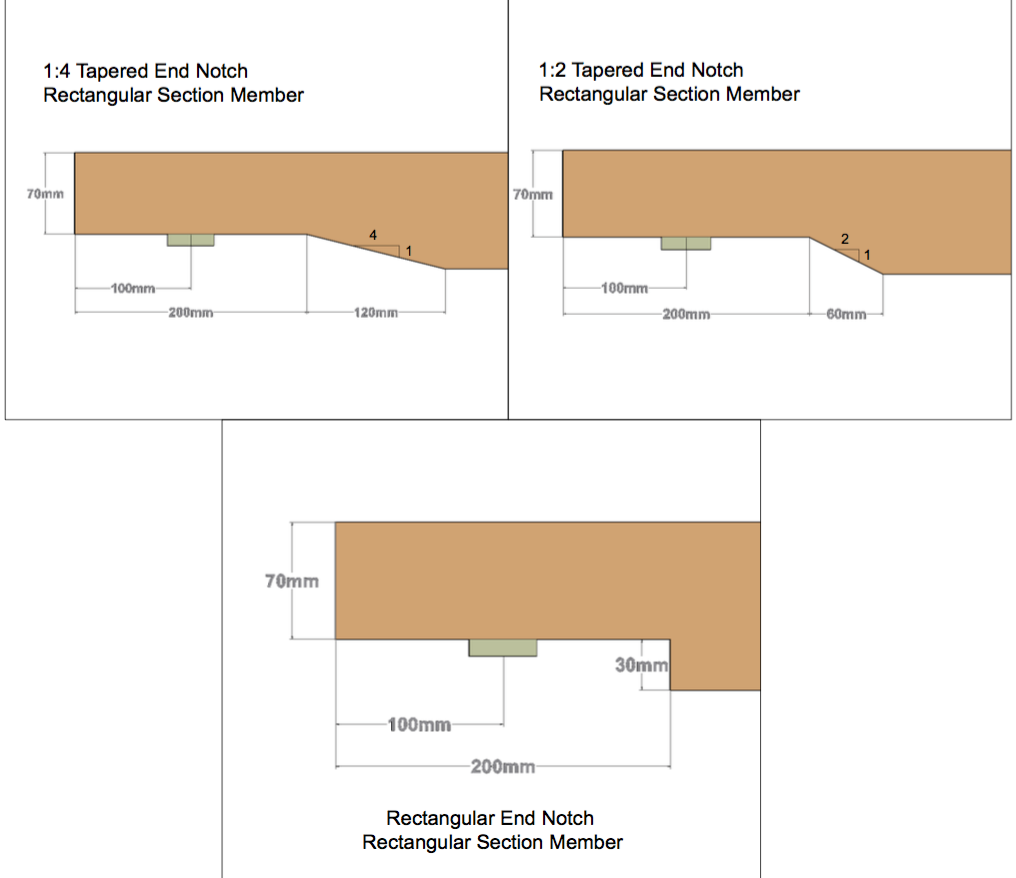
\includegraphics[scale=0.25]{Notch_Angles}
	\end{center}
	\caption{Notch Profiles for Rectangular Section Members}
	\label{fig:Rectangular2}
\end{figure}
\pagebreak

\noindent
A set of 4 specimens for each notch angle in both rectangular and circular section were tested, thus a total of 24 specimens are to were used. The notch layout for each test can be seen in Figures \ref{fig:Rectangular2} and \ref{fig:Circular}. Table 3 shows the set experimental parameters.
\vspace*{\baselineskip}
\begin{figure}[h]
	\begin{center}
		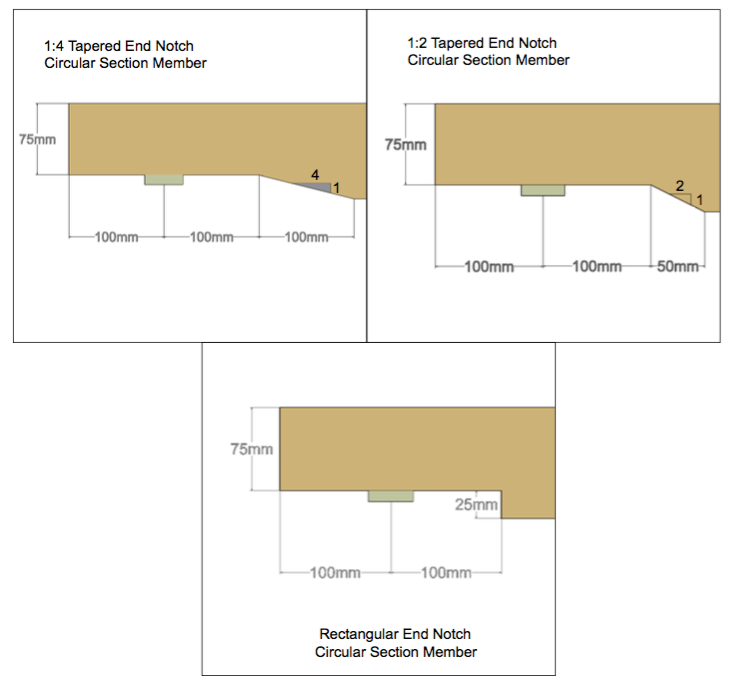
\includegraphics[scale=0.32]{Circular_Notch_Angles}
	\end{center}
	\caption{Notch Profiles for Circular Section Members}
	\label{fig:Circular}
\end{figure}

\pagebreak
\captionof{table}{Notch Altering Parameters}

\begin{center}
	\begin{tabularx}{\textwidth}{|>{\centering}X|>{\centering}X|>{\centering}X|>{\centering}X|>{\centering}X|>{\centering}X|>{\centering}X|>{\centering}X|} 
		\hline
	    \multicolumn{8}{|c|}{Rectangular Section} \\
		\hline
	%	\cline{2-3}
		
		Notch Profile & Notch Angle Slope & Member Depth (m) & Width (m) & Notch Depth (m) & Total Section Area ($10^{-3} m^{2}$) & Notched Corner Area ($10^{-3} m^{2}$) & Moment of Inertia ($10^{-5} m^{4}$) \tabularnewline [0.5ex] 
		\hline
		1 & 1:0 & 0.100 & 0.060 & 0.030 & 6.00 & 4.20 & 5.00 \tabularnewline [0.5ex]
		\hline
		2 & 1:2 & 0.100 & 0.060 & 0.030 & 6.00 & 4.20 & 5.00 \tabularnewline [0.5ex]
		\hline
		3 & 1:4 & 0.100 & 0.060 & 0.030 & 6.00 & 4.20 & 5.00 \tabularnewline [0.5ex]
		\hline
	   
	    \multicolumn{8}{|c|}{Circular Section} \\
	    \hline
	    %	\cline{2-3}
	    
	    Notch Profile & Notch Angle Slope & 
	    \multicolumn{2}{c|}{Diameter (m)}
	    & Notch Depth (m) & Total Section Area ($10^{-3} m^{2}$) & Notched Corner Area ($10^{-3} m^{2}$) & Moment of Inertia ($10^{-5} m^{4}$) \tabularnewline [0.5ex] 
	    \hline
	    1 & 1:0 & \multicolumn{2}{c|}{0.100} & 0.025 & 7.85 & 6.32 & 4.91 \tabularnewline [0.5ex]
	    \hline
	    2 & 1:2 & \multicolumn{2}{c|}{0.100} & 0.025 & 7.85 & 6.32 & 4.91 \tabularnewline [0.5ex]
	    \hline
	    3 & 1:4 & \multicolumn{2}{c|}{0.100} & 0.025 & 7.85 & 6.32 & 4.91 \tabularnewline [0.5ex]
	    \hline
	\end{tabularx}
\end{center}

\vspace*{\baselineskip}

\subsection{Finite Element Analysis}
Finite element analysis (FEA) was completed on ANSYS V17.0 to compare theoretical effects of the experiments with actual results, as well as allow the observation of experimental effects on large scale models. 

\vspace*{\baselineskip}

\noindent
The properties used for the FEA modelling in ANSYS can  be seen in Figure \ref{fig:Properties} below.


	\begin{figure}[h]
		\begin{center}
		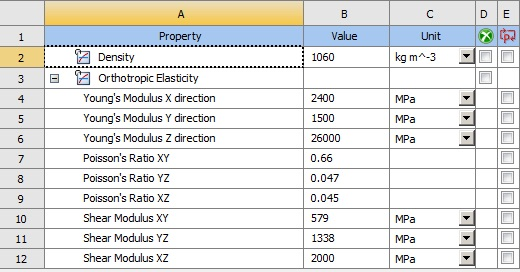
\includegraphics[scale=0.8]{Ansys_Properties}
	\end{center}
		\caption{Rectangular Section Beam: Deflection}
		\label{fig:Properties}
	\end{figure}
\pagebreak


\subsection{Materials}
\noindent \textbf{Timber Properties}\par
\noindent
The timber used for testing was spotted gum (corymbia maculata) timber as it is a prominent timber in Queensland bridge construction. The properties and characteristics of spotted gum timber are given in Table \ref{tab:spotty} \cite{elsener_material_2014,hopewell_spotted_2004}. All specimens will be unseasoned and green (have a water content greater than 12\%).

\vspace*{\baselineskip}

\captionof{table}{Properties of Spotted Gum (Corymbia Maculata) \cite{elsener_material_2014,hopewell_spotted_2004}}
\label{tab:spotty}

\begin{center}
	\begin{tabularx}{\textwidth}{|>{\centering}X|>{\centering}X|>{\centering}X|>{\centering}X|>{\centering}X|}	
		\hline 
		
		\multicolumn{2}{|c|}{\textbf{Properties}} & \textbf{Moisture Content 12\%} & \textbf{Green (MC $\textgreater$ 12\%)}  & \textbf{Dry (MC $\textless$ 12\%)} \tabularnewline  [0.5ex]
		\hline
		
		\multirow{3}{*}{\parbox{2.5cm}{\centering Modulus of Rupture MOR (MPa)}}& \textit{Longitudinal} & 141.1 & 99 & 150 \tabularnewline  [0.5ex] 
		\cline{2-5}
		& \textit{Radial} & 19.5 &  &  \tabularnewline [0.5ex] 
		\cline{2-5}
		& \textit{Tangential} & 14.9 &  &  \tabularnewline [0.5ex] 
		\hline
		
		\multirow{3}{*}{\parbox{2.5cm}{\centering Modulus of Elasticity MOE (MPa)}} & \textit{Longitudinal} & 26174 & 18000 & 23000 \tabularnewline [0.5ex] 
		\cline{2-5}
		& \textit{Radial} & 2405 & 1531 &  \tabularnewline [0.5ex] 
		\cline{2-5}
		& \textit{Tangential} & 1499 & 665 &  \tabularnewline [0.5ex] 
		\hline
		
		\multirow{3}{*}{\parbox{2.5cm}{\centering Shear Modulus G (MPa)}}& \textit{Long - Rad} & 1736 &  &  \tabularnewline [0.5ex] 
		\cline{2-5}
		& \textit{Rad - Tang} & 840 &  &  \tabularnewline [0.5ex] 
		\cline{2-5}
		& \textit{Long - Tang} & 1530 &  &  \tabularnewline [0.5ex] 
		\hline
		
		\multirow{6}{*}{\parbox{2.5cm}{\centering Poisson's Ratio $\nu$}}& \textit{Long - Rad} & 0.49 &  &  \tabularnewline [0.5ex] 
		\cline{2-5}
		& \textit{Long - Tang} & 0.550 &  &  \tabularnewline [0.5ex] 
		\cline{2-5}
		& \textit{Rad - Tang} & 0.660 & 0.660 &  \tabularnewline [0.5ex] 
		\cline{2-5}
		& \textit{Rad - Long} & 0.045 & 0.040 &  \tabularnewline [0.5ex] 
		\cline{2-5}
		& \textit{Tang - Rad} & 0.480 &  &  \tabularnewline [0.5ex] 
		\cline{2-5}
		& \textit{Tang - Long} & 0.047 & 0.050 &  \tabularnewline [0.5ex] 
		\hline
		
		
		\multicolumn{2}{|c|}{Bending Strength (MPa)}& 142 &  &   \tabularnewline [0.5ex] 
		\hline
		
		\multicolumn{2}{|c|}{Compressive Strength (MPa)}& 76 &  &   \tabularnewline [0.5ex] 
		\hline
		
		\multicolumn{2}{|c|}{Tensile Strength (MPa)}& 159 &  &   \tabularnewline [0.5ex] 
		\hline
		
		\multicolumn{2}{|c|}{Density ($kg/m^{3}$)}& 1060 & 1150 & 1100  \tabularnewline [0.5ex] 
		\hline
		
		\multicolumn{2}{|c|}{Strength Group}&  & S2 & SD2  \tabularnewline [0.5ex] 
		\hline
		
		\multicolumn{2}{|c|}{F-Grade}&  & F14 & F22  \tabularnewline [0.5ex] 
		\hline
		
	\end{tabularx}
\end{center}

\vspace*{\baselineskip}
\noindent \textbf{Strain Gauges}\par

\subsection{Methodology}

\textbf{Specimen Documentation}\par
\noindent
Before any testing was undertaken, the specimens were required to be documented in great detail, to account for any inaccuracies or defect interference with experimental results. Firstly, the length, width, depth, average diameter, notch length, notch depth and mass were measured and recorded. After the mass and all required dimensions were taken, the specimen was carefully checked for defects and imperfections (i.e. knots, rot, cracks etc.), which were measured, photographed and documented. This process was repeated for all 24 specimens. 

\vspace*{\baselineskip}

\textbf{Specimen Strain Gauge Implementation}\par
\noindent
To prepare for the strain gauges to be adhered to a specimen, each specimen was measured and marked on their top and bottom faces at the centre of the beam, and 5mm vertically and horizontally from the notch corner, to show the intended gauge placements. After this, a 10mm strain gauge (FRA--3--350--11--1L) was centrally placed on the marking in the middle of the top and bottom face of the beam using epoxy adhesive, running along the grain. Strain gauges of 2mm and 10mm were placed near the notch corner as marked on either side of the specimen. If the wires from a strain gauge were touching, they separated using duct tape. The strain gauges were arranged and properly attached to specimens between experiments.

\vspace*{\baselineskip}

\textbf{LVDT Implementation}\par
\noindent
For the rectangular specimens, a 20cm long, 2cm wide and 5mm thick piece of plywood was attached to the specimen and mid-span using super glue. Once it was dry and secured, a 50mm LDVT was magnetically attached to the MTS machine and placed directly above the piece of plywood. For the round specimens, a long metal plate was incorporated into the constructed curved loading plate, which levelly extruded from the centre of the beam to allow seating for the LVDT.

\vspace*{\baselineskip}

\textbf{Timber Specimen Test Set-Up}\par
\noindent
Once the strain gauges had been securely attached to a specimen, the specimen was ready to be set-up to undertake loading. To set-up the experiment, the timber specimen was placed upon a simply supported arrangement within the MTS machine. This arrangement consisted of the notched end supported by a pin support and un-notched end supported by a roller, with a span of 600mm between supports. The metal support plates were then slipped under the member to sit centrally above the two end supports, with extreme care taken to not pull on any strain gauges throughout the set-up. 

\vspace*{\baselineskip}

\textbf{Data Logger Set Up}\par
\noindent
After the specimen experimental arrangement was complete, the strain gauges were connected to the data logger. This was achieved by wiring 8 ports of the data logger with long wires that had alligator clips at the opposing ends. These ports were numbered 1 to 8; where wires 1 to 6 were clipped onto specific strain gauges attached to the specimen, wire 7 was clipped onto the LVDT and wire 8 was clipped onto the loading cell. The alligator clips were unattached after the completion of each experiment and were ready to be reattached when the next specimen was set-up. 

\vspace*{\baselineskip}

\textbf{Timber Specimen Testing}\par
\noindent
Once the specimen was correctly placed, set-up and all strain gauges and the LVDT was connected, the load cell was placed on top of the loading plate, steel disc and steel ball. A 5mm x 100mm x 100mm steel loading plate was then placed on top of the load cell, and the MTS load was lowered until it was just touching the top loading plate. Before we began loading, the data logger readings from the strain gauges, LVDT and load cell were checked to determine if all were properly connected and collecting data. Finally a load was applied at a constant rate, by the MTS machine, until the specimen failed. 

\vspace*{\baselineskip}
\noindent
The steps described in the specimen strain gauge implementation, LVDT implementation, timber specimen test set-up, data logger set up and timber specimen testing were repeated for all 24 specimens. 


\pagebreak

\section{Results}

\subsection{Rectangular Specimens}
\vspace*{\baselineskip}
\noindent Compiled graphs showing exact data from results for load displacement, centre tension, centre compression, z-stress and y-stress \par

\vspace*{\baselineskip}
\noindent Table showing cracking and ultimate loads and times \par

\vspace*{\baselineskip}
\noindent Graph showing exact loading rates \par

\vspace*{\baselineskip}
\noindent Graph showing water content vs. notch cracking load and ultimate failure load \par

\subsection{Round Specimens}
\vspace*{\baselineskip}
\noindent Compiled graphs showing exact data from results for load displacement, centre tension, centre compression, z-stress and y-stress \par

\vspace*{\baselineskip}
\noindent Table showing cracking and ultimate loads and times \par

\vspace*{\baselineskip}
\noindent Graph showing exact loading rates \par

\vspace*{\baselineskip}
\noindent Graph showing water content vs. notch cracking load and ultimate failure load \par

\subsection{Predicted Capacities using Standards}

\vspace*{\baselineskip}
\noindent Tables with predicted capacities from AS1720, Eurocode 5 and CSA O.86\par

\subsection{Finite Element Analysis}
\noindent
A small scale ANSYS model has also been established to determine the optimum placement for data reading equipment and critical loading set-out for all tests. Figures \ref{fig:Def} to \ref{fig:fig:y_norm} show the ANSYS analysis for the rectangular end notched specimen, centrally loaded and simply supported.

\vspace*{\baselineskip}

\begin{figure}[h]
	\begin{center}
		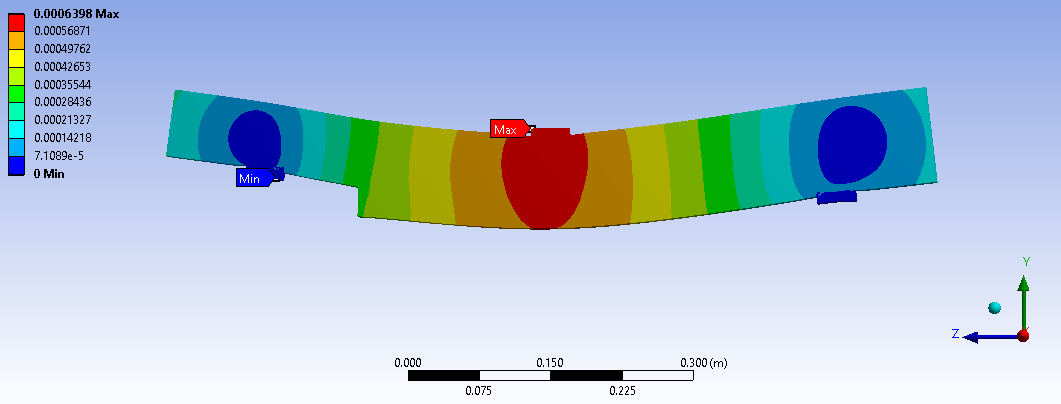
\includegraphics[scale=0.45]{Ansys_Deflection}
	\end{center}
	
	\caption{Rectangular Section Beam: Deflection}
	\label{fig:Def}
\end{figure}
\pagebreak

\begin{figure}[h]
	\begin{center}
		\includegraphics[scale=0.45]{YZ_shear_strain}
	\end{center}
	\caption{Rectangular Section Beam: XY-Plane Shear Strain}
	\label{fig:yz_shear}
\end{figure}

\begin{figure}[h]
	\begin{center}
		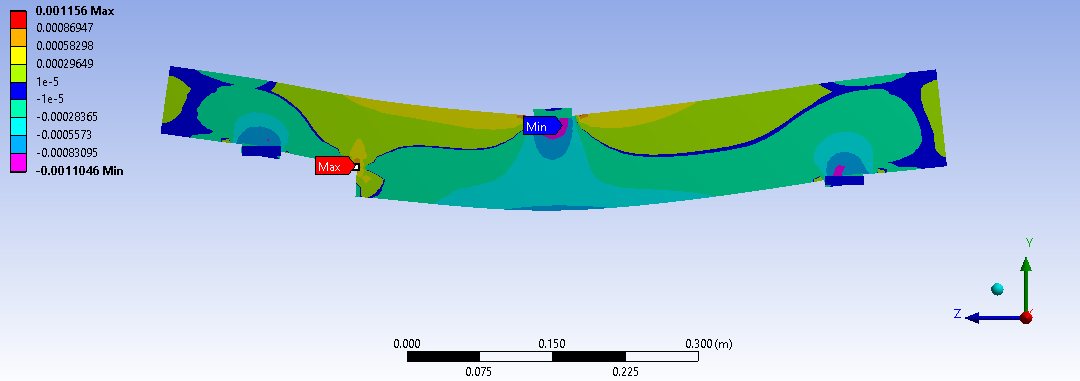
\includegraphics[scale=0.45]{y_normal_strain}
		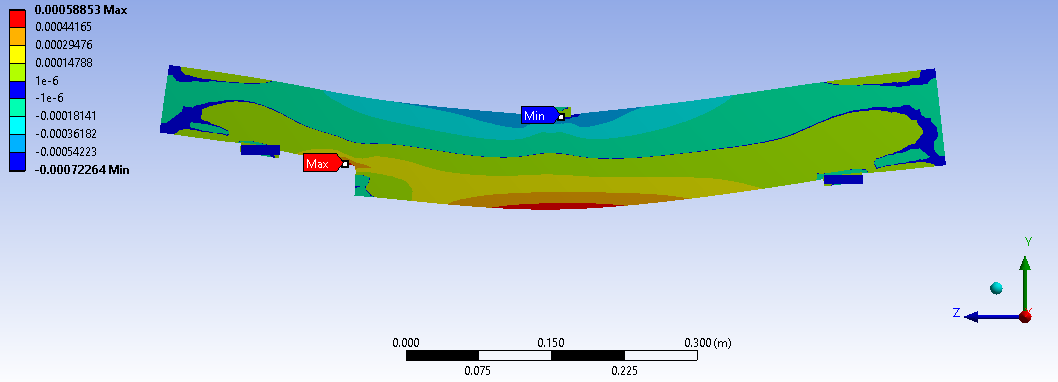
\includegraphics[scale=0.45]{z_normal_strain}
	\end{center}
	\caption{Rectangular Section Beam: Normal Strain in Y-direction (upper) and Z-direction (lower)}
	\label{fig:fig:y_norm}
\end{figure}
\pagebreak
\vspace*{\baselineskip}  


\section{Discussion}

\vspace*{\baselineskip}
\noindent Trends in rectangular and round specimen results (noting the critical angle, failure modes and time between crack initiation and ultimate failure) \par

\vspace*{\baselineskip}
\noindent Discuss variance in results relating to water contents and existing defects, refer to Appendix A \par

\vspace*{\baselineskip}
\noindent Discuss/determine a relationship between rectangular and round specimens\par

\vspace*{\baselineskip}
\noindent Look into round design and apply the new As for the notched end to see results and maybe discuss a factor for a notched member\par

\vspace*{\baselineskip}
\noindent Include and discuss graphs comparing the results to predicted capacities from Australian Standards, Eurocode 5 and CSA O.86. Discuss which design yields the best results and why. \par

\vspace*{\baselineskip}
\noindent Compare actual strain/stress results with ANSYS results at the untimate failure load\par

\pagebreak	


\section{Conclusions}
\vspace*{\baselineskip}
\noindent Concluded which was the critical angle, most common failure modes and time between crack initiation and ultimate failure for both rectangular and round specimens\par

\vspace*{\baselineskip}
\noindent Was a relationship between rectangular and round specimens determined? What was it/why not?\par

\vspace*{\baselineskip}
\noindent Which code yielded the best results\par

\vspace*{\baselineskip}
\noindent Was the finite element analysis accurate in comparison to actual results?\par

\pagebreak	

\bibliographystyle{unsrt}
\bibliography{My_Library.bib}

\pagebreak
\cleardoublepage
\pagenumbering{gobble}

\appendixtitleon

\begin{appendices}
	\section{\textit{Specimen Characteristics}}
\pagebreak

\thispagestyle{empty}	
	\begin{sidewaystable}
		\footnotesize
		\centering
	\begin{tabularx}{\textwidth}{|>{\centering}X|>{\centering}X|>{\centering}X|>{\centering}X|>{\centering}X|>{\centering}X|>{\centering}X|>{\centering}X|>{\centering}X|>{\centering}X|}  
		\hline
		
		\multicolumn{10}{|c|}{\textbf{Rectangular Section}} \\
		\hline \hline
		
		Specimen Number & Notch Slope & Mass (kg) & Total Length (mm) & Average Width (mm) & Length to Chamfer (mm) & Length of Chamfer (mm) & Average Total Depth (mm) & Average Depth Above Notch (mm) & Comments 
		\tabularnewline [0.5ex] 
		\hline
		1 & 1:0 & 4.680 & 798.0 & 58.80 & 201.0 & N/A & 96.93 & 66.90 & Knot on bottom approx. 200mm from unnotched end, spans 80mm length and 45mm wide. 1mm wide, 13mm deep drying crack on centre LHS above notch, spanning from notch end to half way along beam.
		\tabularnewline [0.5ex]
		\hline
		2 & 1:0 & 5.085 & 801.5 & 59.70 & 201.0 & N/A & 96.71 & 67.44 & 3mm deep wedge cut from notched end. Spans 19mm length and 37mm width. 
		\tabularnewline [0.5ex]
		\hline
		3 & 1:0 & 4.800 & 797.5 & 61.40 & 200.0 & N/A & 97.15 & 65.76 & 1mm wide, 15mm deep drying crack on centre LHS above notch, spanning from notch end to half way along beam.
		\tabularnewline [0.5ex]
		\hline
		4 & 1:0 & 4.665 & 801.5 & 58.90 & 199.8 & N/A & 96.43 & 66.59 & 1.5mm deep lip on RHS bottom of unnotched end. Spans length of 29.8mm and 2.8 width.
		\tabularnewline [0.5ex]
		\hline	
	\end{tabularx}
	\end{sidewaystable}

	\begin{sidewaystable}
		\footnotesize
		\centering
		\begin{tabularx}{\textwidth}{|>{\centering}X|>{\centering}X|>{\centering}X|>{\centering}X|>{\centering}X|>{\centering}X|>{\centering}X|>{\centering}X|>{\centering}X|>{\centering}X|}  
			\hline
			
			\multicolumn{10}{|c|}{\textbf{Rectangular Section}} \\
			\hline \hline
			
			Specimen Number & Notch Slope & Mass (kg) & Total Length (mm) & Average Width (mm) & Length to Chamfer (mm) & Length of Chamfer (mm) & Average Total Depth (mm) & Average Depth Above Notch (mm) & Comments 
			\tabularnewline [0.5ex] 
			\hline
			1 & 1:2 & 4.630 & 800.0 & 59.10 & 200.0 & 62.70 & 96.99 & 67.86 & No defects
			\tabularnewline [0.5ex]
			\hline
			2 & 1:2 & 4.665 & 801.0 & 58.30 & 202.0 & 65.50 & 96.49 & 67.65 & 1mm thick cut 8.5mm length from notched end. 
			\tabularnewline [0.5ex]
			\hline
			3 & 1:2 & 4.880 & 802.0 & 59.30 & 205.0 & 67.50 & 96.92 & 66.97 & 1mm deep notch cut top LHS notch corner.
			\tabularnewline [0.5ex]
			\hline
			4 & 1:2 & 4.645 & 800.0 & 59.20 & 199.5 & 60.60 & 96.96 & 69.07 & No defects
			\tabularnewline [0.5ex]
			\hline	
			
			1 & 1:4 & 4.695 & 800.5 & 59.90 & 200.8 & 118.4 & 96.68 & 66.92 & No defects
			\tabularnewline [0.5ex]
			\hline
			2 & 1:4 & 5.145 & 800.0 & 60.00 & 200.4 & 122.8 & 97.11 & 66.88 & Shallow crack from unnotched end. 255mm length and 0.5mm width. 28.8mm deep crack from notched end, 1mm width and 42.1mm length.
			\tabularnewline [0.5ex]
			\hline
			3 & 1:4 & 4.830 & 799.50 & 58.80 & 201.5 & 121.4 & 96.92 & 69.23 & No defects
			\tabularnewline [0.5ex]
			\hline
			4 & 1:4 & 4.910 & 800.5 & 60.90 & 199.4 & 121.3 & 96.08 & 65.22 & 1mm deep notch cut top RHS notch corner.
			\tabularnewline [0.5ex]
			\hline	
		\end{tabularx}
	\end{sidewaystable}
	
	\begin{sidewaystable}
		\footnotesize
		\centering
		\begin{tabularx}{\textwidth}{|>{\centering}X|>{\centering}X|>{\centering}X|>{\centering}X|>{\centering}X|>{\centering}X|>{\centering}X|>{\centering}X|>{\centering}X|>{\centering}X|>{\centering}X|}  
				\hline
				
			\multicolumn{11}{|c|}{\textbf{Round Section}} \\
				\hline \hline
				
			Specimen Number & Notch Slope & Mass (kg) & Total Length (mm) & Average Diameter (mm) & Length to Chamfer (mm) & Length of Chamfer (mm) & Depth Above Notch (mm) & Length of Support Section (mm) & Depth Above Support Section (mm) & Comments 
			\tabularnewline [0.5ex] 
			\hline
			1 & 1:0 & 7.000 & 799.0 & 101.2 & 200.9 & N/A & 76.00 & 128.7 & 89.10 & Numerous 1mm wide, 5mm deep drying cracks running full length on LHS and bottom of beam. 2mm wide, 31.7 deep drying crack on flat of notched end, running to notched corner.
			\tabularnewline [0.5ex]
			\hline
			2 & 1:0 & 6.595 & 798.5 & 99.20 & 200.6 & N/A & 76.30 & 127.70 & 90.00 & Hairling crack, 10mm long from notch corner LHS. No drying cracks. Shallow 550mm shaving along LHS starting from notched end. 
			\tabularnewline [0.5ex]
			\hline
			3 & 1:0 & 6.925 & 800.0 & 99.40 & 199.9 & N/A & 76.40 & 131.0 & 91.20 & 8mm deep hairline crack from LHS notch corner. 153mmx48mm gum vein, top of member, support end. 1mm thick drying crack, spans full length LHS. Numerous 1mm thick drying cracks around member.
			\tabularnewline [0.5ex]
			\hline
			\end{tabularx}
		\end{sidewaystable}
	
	\begin{sidewaystable}
		\footnotesize
		\centering	
		\begin{tabularx}{\textwidth}{|>{\centering}X|>{\centering}X|>{\centering}X|>{\centering}X|>{\centering}X|>{\centering}X|>{\centering}X|>{\centering}X|>{\centering}X|>{\centering}X|>{\centering}X|} 
			\hline
			
			\multicolumn{11}{|c|}{\textbf{Round Section}} \\
			\hline \hline
			
			Specimen Number & Notch Slope & Mass (kg) & Total Length (mm) & Average Diameter (mm) & Length to Chamfer (mm) & Length of Chamfer (mm) & Depth Above Notch (mm) & Length of Support Section (mm) & Depth Above Support Section (mm) & Comments 
			\tabularnewline [0.5ex] 
			\hline
			4 & 1:0 & 6.475 & 799.0 & 99.10 & 200.5 & N/A & 71.50 & 129.2 & 88.00 & 10mmx1mm rot 12mm from centre section, support end. 21mm deep, 1mm wide drying crack, from centre end to corner of support. 13.5mm deep, 1.5mm thick drying crack, centre end to notch corner. Numerous 0.5mm wide drying cracks all around member. 0.5mm Drying cracks at both notch corners.
			\tabularnewline [0.5ex]
			\hline	
			1 & 1:2 & 6.775 & 798.0 & 100.7 & 199.3 & 54.10 & 75.40 & 130.6 & 89.50 & Shallow 400mm shaving along RHS starting 1/16 in from notched end. 69mm deep, 1mm thick drying crack, running 1/16 on flat from notch end, crack through crentre of section. Numerous 1mm thick drying cracks on LHS and bottom. 11.8mmx2mm rot at support end, origination from centre of section. 11.1mmx8.2mm knot, 9/16 LHS from notched end. 6.9mmx6.1mm knot 1/4 in from support end, LHS. 
			\tabularnewline [0.5ex]
			\hline
			2 & 1:2 & 6.765 & 799.0 & 101.0 & 200.3 & 54.00 & 74.20 & 128.4 & 89.60 & 10mmx8.3mm knot at 1/8 in on notch flat. 7.2mmx12.8mm knot at RHS notch corner.2mm wide, 18.7mm deep longitinal drying crack, spanning 1/8 from support end, RHS. Numerous drying cracks 0.5mm wide and 18mm deep cracking toward core. 
			\tabularnewline [0.5ex]
			\hline

		\end{tabularx}
		\end{sidewaystable}
	
\end{appendices}


\end{document}
